%%%%%%%%%%%%%%%%%%%%%%% file template.tex %%%%%%%%%%%%%%%%%%%%%%%%%
%
% This is a template file for Web of Conferences Journal
%
% Copy it to a new file with a new name and use it as the basis
% for your article
%
%%%%%%%%%%%%%%%%%%%%%%%%%% EDP Science %%%%%%%%%%%%%%%%%%%%%%%%%%%%
%
%%%\documentclass[option]{webofc}
%%% "twocolumn" for typesetting an article in two columns format (default one column)
%

\newcommand{\sqrts}{\ensuremath{\sqrt{s}}\xspace}
\newcommand{\sqrtsNN}{\ensuremath{\sqrt{\smash[b]{s_{_{\text{NN}}}}}}\xspace}
\newcommand{\PbPb}{\ensuremath{\mathrm{PbPb}}\xspace}
\newcommand{\pp}{\ensuremath{\Pp\Pp}\xspace}
\newcommand{\raa}{\ensuremath{R_{\mathrm{AA}}}\xspace}
\newcommand{\rpa}{\ensuremath{R_{p \mathrm{A}}}\xspace}
\newcommand{\taa}{\ensuremath{T_{\mathrm{AA}}}\xspace}
\newcommand{\absy}{\ensuremath{ \abs{y}}\xspace}
\newcommand{\abseta}{\ensuremath{ \abs{\eta}}\xspace}
\newcommand{\Dzero}{\rm D^{0}\xspace}
\newcommand{\Bplus}{\rm B^{+}\xspace}
\newcommand{\Dzerodecay}{\rm D^{0} \rightarrow K^{-} \pi^{+}\xspace}
\newcommand{\Bplusdecay}{\rm \Bplus \rightarrow J/\Psi \hspace{0.1cm} K^{+} \rightarrow \mu^{+} \mu^{+} K^{+}}
\newcommand{\bdecayX}{\rm B \rightarrow J/\Psi \hspace{0.1cm} X}
\newcommand{\Ds}{\rm D_{s}^{+}\xspace}
\newcommand{\Lambdac}{\rm \Lambda_{c}\xspace}
\newcommand{\pt}{\rm p_{\rm T} \xspace}

\documentclass{webofc}
\usepackage[varg]{txfonts}   % Web of Conferences font
%
% Put here some packages required or/and some personnal commands
%
%
\begin{document}
%
\title{Heavy flavour production at RHIC and LHC}
%
% subtitle is optionnal
%
%%%\subtitle{Do you have a subtitle?\\ If so, write it here}

\author{\firstname{Gian Michele} \lastname{Innocenti}\inst{1}\fnsep\thanks{\email{ginnocen@cern.ch}} 
}

\institute{Massachusetts Institute of Technology}

\abstract{
In this proceedings, I present selected experimental results on heavy-flavour production at RHIC and at the LHC, which were 
presented at the Strangeness in Quark Matter 2017 conference. I will present a brief introduction to the heavy-flavour physics in 
heavy ion collisions and I will focus on recents measurements of in-medium energy loss and and collective properties of  heavy-flavour  
particles, which provided relevant information on the mechanisms of heavy flavour interaction with the hot and dense medium 
created in ultra-relativistic heavy-ion collisions. I will also briefly discuss the open physics questions in our field and 
my personal view on the future and the challenges of heavy flavour measurements at RHIC and at the LHC.
}
%
\maketitle
%
\section{Introduction}
\label{intro}
Heavy quarks are effective probes to study the properties of the deconfined medium created in heavy ion collisions (more details and a complete bibliography can 
be found in~\cite{saporegravis}). These quarks, as a consequence of their large masses, are mostly produced in primary hard QCD scatterings with a production timescale that is shorter than the formation time of the 
QGP. During their propagation through the medium, heavy quarks lose energy via radiative and collisional 
interactions with the medium constituents. Through the interactions with light partons and gluons, heavy quarks are also expected to be dragged in the collective 
expansion of the medium. By studying the effects of in-medium energy loss phenomena and the collective properties of heavy-flavoured particles, 
one can obtain important information on the mechanisms of heavy-quark interaction with the medium and derive fundamental properties like the medium density 
and the diffusion coefficients. Quarks are expected to lose less energy than gluons as a consequence of their smaller colour factor. 
In addition, the so-called ``dead-cone effect" is expected to reduce small-angle gluon radiation of heavy quarks when compared to both 
gluons and light quarks.  Energy loss can be studied using the nuclear modification factor (\raa), defined as the ratio of the PbPb yield to the pp cross-section scaled by 
the nuclear overlap function. Precise measurements of the \raa of particles containing both light and heavy quarks can thus 
provide important tests of QCD predictions at extreme densities and temperatures. The measurement of the \raa of strange D mesons 
can also help to estimate the relevance of the coalescence mechanism in which charmed hadrons are formed 
by the combination of charm quarks with light quarks from the medium. If coalescence plays a relevant role in the charm hadronisation, 
the yield of $\Ds$ particles are expected to be significantly enhanced with respect to $\Dzero$ at low transverse momenta, 
as a consequence of the increased abundance of strange quarks in the deconfined medium. The production ratio of $\Lambdac/\Dzero$ 
is also expected to be enhanced with respect to that of charmed mesons under the assumption that di-quarks bounded states in the 
quark-gluon plasma can be formed. The study of the collective properties of D and B mesons through detailed measurements of their azimuthal coefficienct $v_{n}$ 
at low $\pt$ can also help quantify the extent to which charm and beauty quarks flow with the medium, 
which is a good measure of their interaction strength. These measurements can also provide further constraints on the role of charm 
coalescence, which is expected to increase the values of the D meson $v_{n}$ coefficients.
\\ \\
The production of open heavy-flavour is measured at RHIC and at the LHC using several experimental techniques. Charm and beauty hadrons can me measured via the exclusive reconstruction 
of their hadronic or semi-leptonic decay channels (e.g. $\Dzerodecay$ or $\Bplusdecay$) or via the inclusive reconstruction of semi-leptonic decays (e.g. $\bdecayX$). The production of 
heavy-flavour particles can also be studied up to very high $\pt$ by measuring jets of hadrons produced in the fragmentation of a charm or beauty quark.  Charm and beauty decays are 
characterised by relativetely small cross sections and by decay vertices which are displaced few hundreds $\mu$m from the main interaction vertices.
Therefore the study of these observables require very large statistics of minimum-bias and triggered events 
and precise tracking and vertexing detectors that can operate under conditions of very large detector occupancy. 
\section{Proton-proton measurements}
\label{ppmeasurements}
The study of heavy-flavour production in proton-proton collisions is considered a fundamental reference for nucleus-nucleus measurements but at the same time it provides
an important test for perturbative QCD calculations at RHIC and LHC energies.The possibility of measuring the charm and beauty production with the two accelerators is crucial to constrain the relevance 
of different production mechanisms (e.g. flavour creation vs gluon fusion processes), which are expected to play a different role at the two different energies. The $\pt$- and $y$-differential cross sections of charm and beauty quarks were 
measured by several collaborations at the two accelerators and were found to be consistent with perturbative QCD calculations (e.g. FONLL) that include a consistent description of next-to-leading order processes. 
As an example, in the left panel of Fig.~\ref{fig:ppresults}, the $\Dzero$ production cross sections as a function of $\pt$ measured by the ALICE experiment at LHC at 7 TeV and by the STAR experiment at RHIC at 200 and 500 GeV are presented. 
In the central panel of the same figure, the $\Bplus$ production measured by the ATLAS  experiment at 7 TeV. Although theoretical calculations showed to be able to describe successfully single-differential 
observables, more differential measurements like $\rm D \bar{D}$ or $\rm B \bar{B}$ azimuthal correlations showed that the current understanding of next-to-leading order processes at the LHC is still not satisfactory. In particular, 
the contribution of the gluon-splitting production mechanism ($g \rightarrow c\bar{c}$ or $g \rightarrow b\bar{b}$), which is dominant at small angles between the particle-anti-particle pairs is 
sizeably understimated by the calculations that can provide results for more-differential observables (right panel of Fig.~\ref{fig:ppresults}). As it will be discussed in the next sections, a proper descriptions of the different type of production 
mechanisms in theoretical calculations is fundamental to guarantee a precise understanding of energy-loss phenomena in heavy-ion collisions. 
\begin{figure}[ht]
\centering
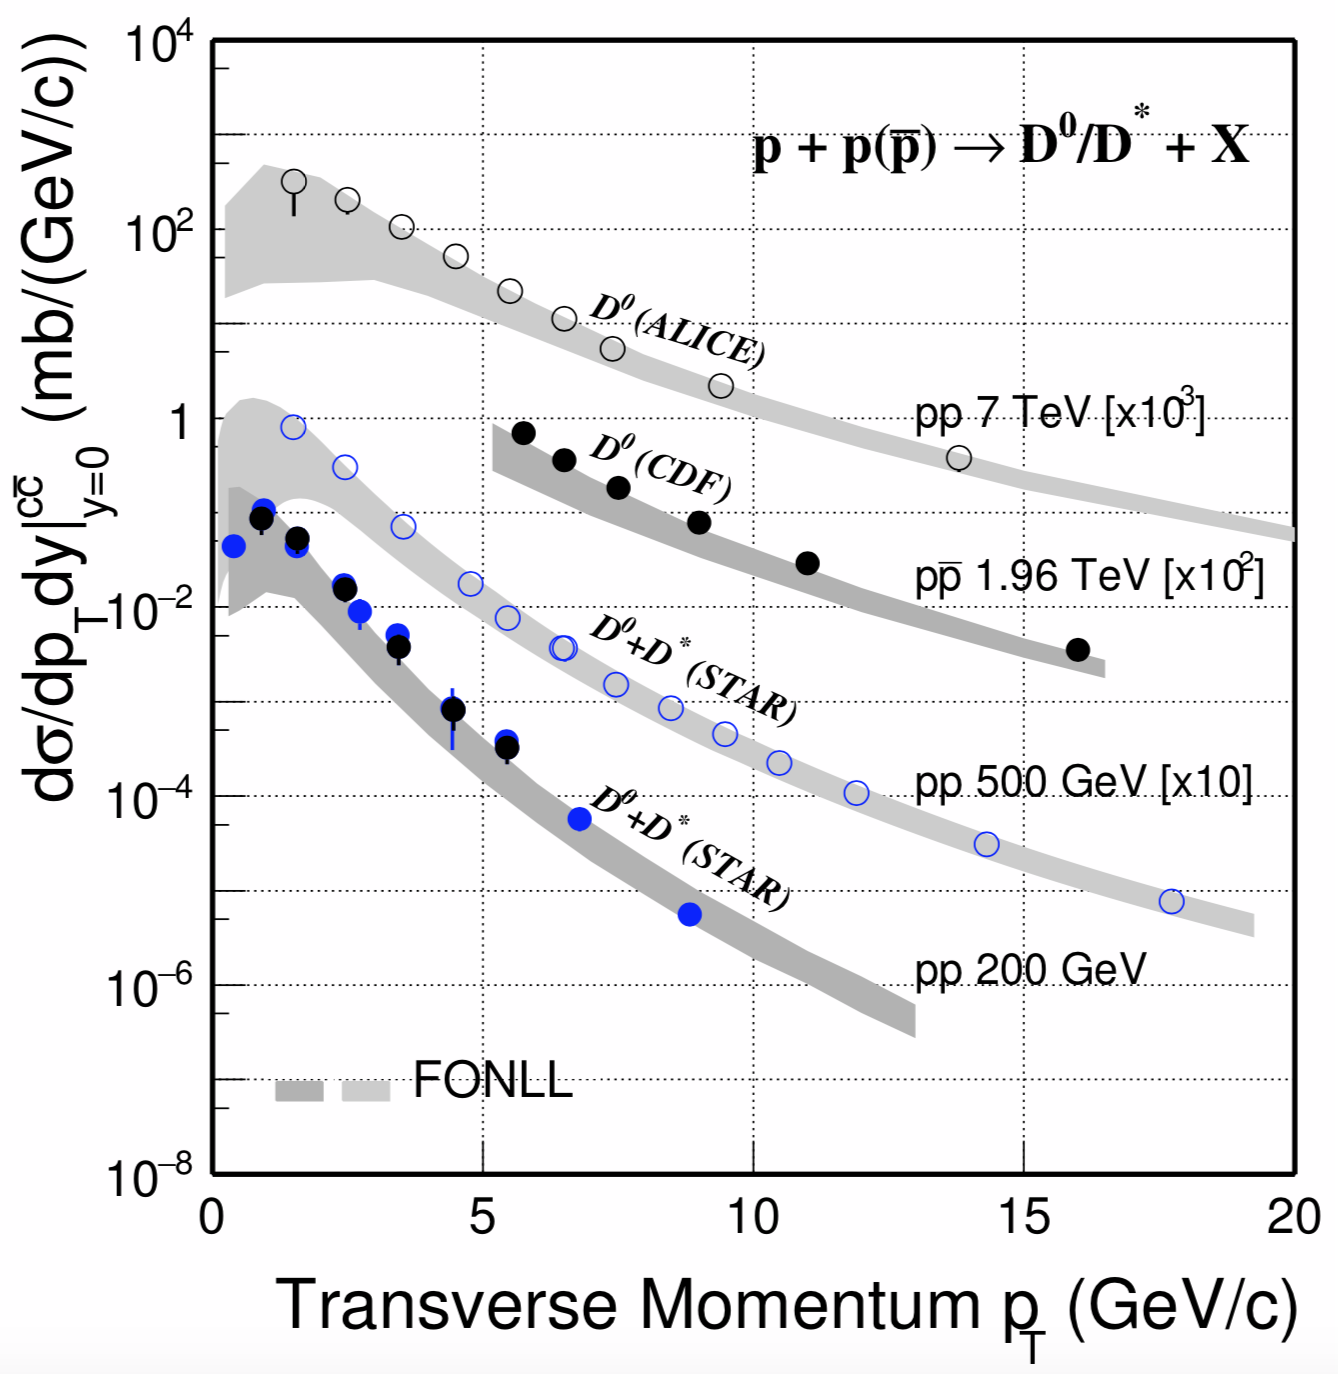
\includegraphics[width=.32\textwidth]{Plots/Dcross_sectionLHCRHIC}
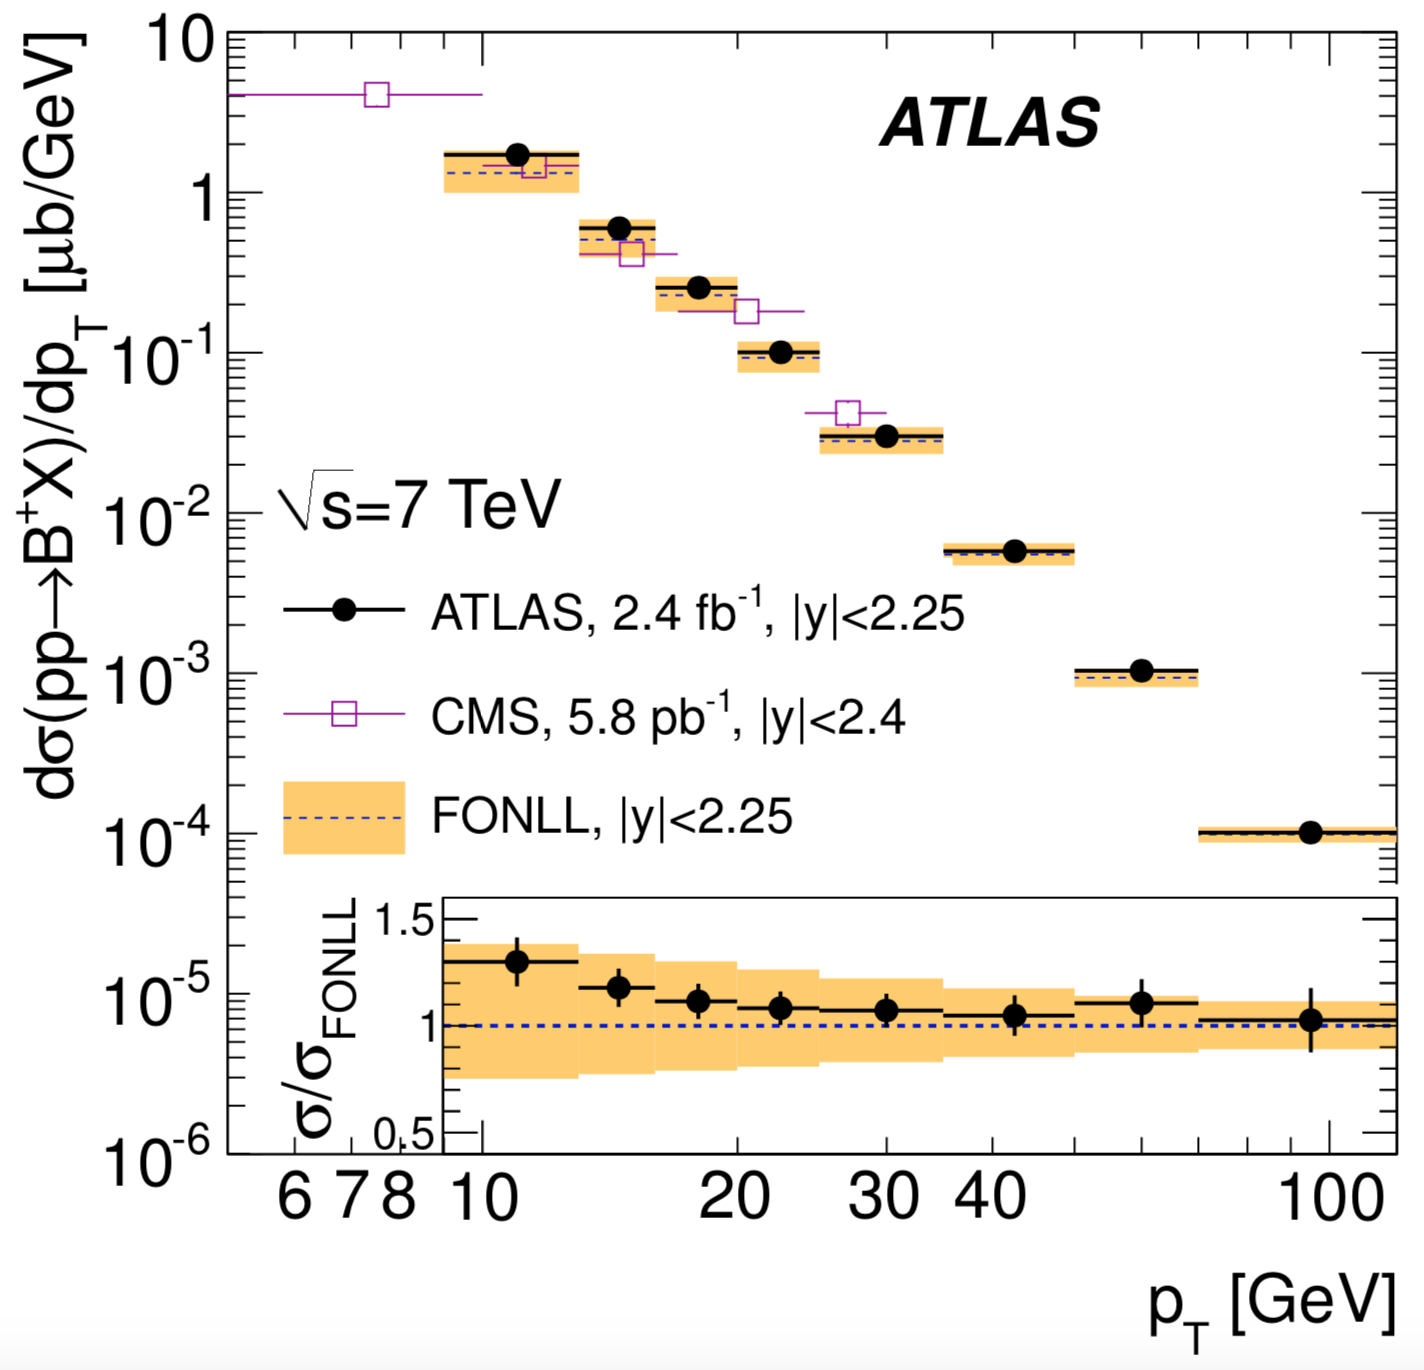
\includegraphics[width=.32\textwidth]{Plots/BplusATLASpp}
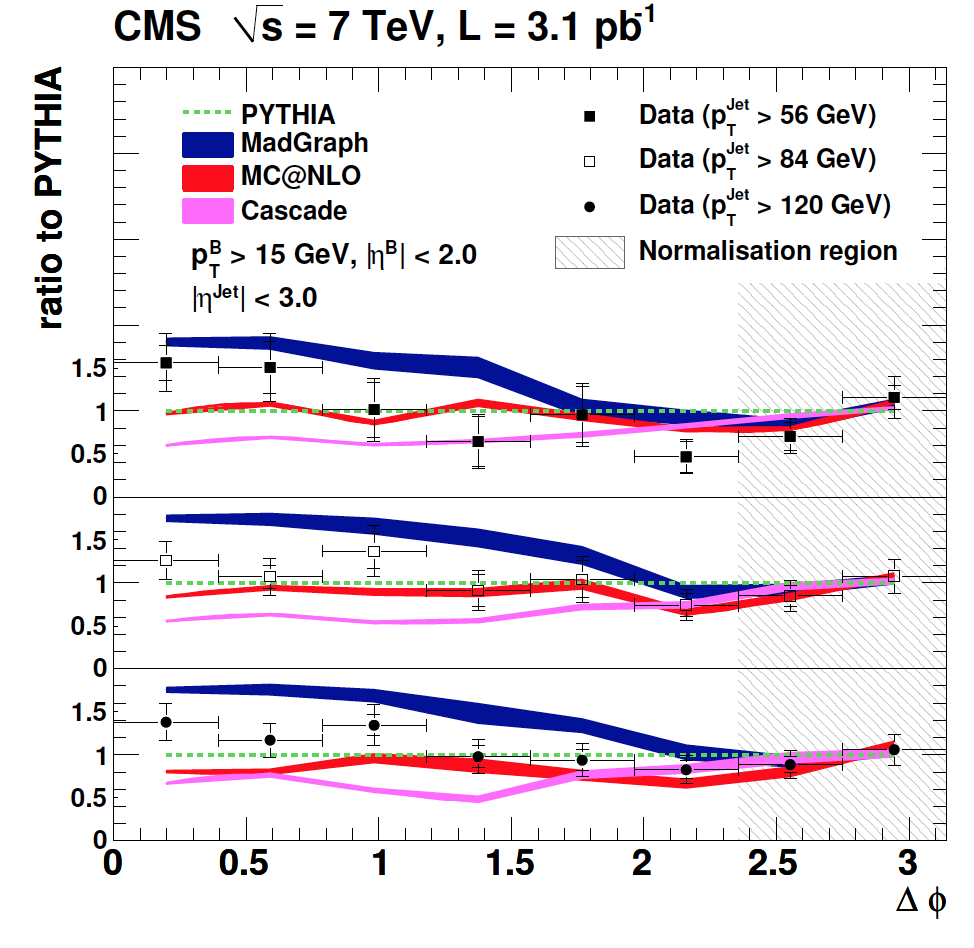
\includegraphics[width=.32\textwidth]{Plots/BBbarCMS7TeV}
\caption{Please write your figure caption here}
\label{fig:ppresults}     
\end{figure}


\section{Proton-nucleus measurements}
\label{ppmeasurements}
In presence of a nuclear environment, the yield of production of light and heavy particles can be modified in absence of any deconfined medium (initial or cold nuclear matter effects). In particular, modifications of the 
parton distribution functions (PDFs) in the nucleus with respect to nucleon PDFs are expected to be responsable for sizeable modifications of the heavy-flavour cross section expecially at 
low transverse momenta. In order to quantify the effects of these phenomena and validate the hypothesis that the suppression observed in nucleus-nucleus collisions is a consequence of the presence of a a hot and dense medium, 
one can quantify these modifications in proton-nucleus collisions where the formation of a hot and dense medium is not expected. In the last years, after exciting LHC measurements have highlighted the presence of 
non-trivial collective phenomena, the role of ``reference'' of proton-nucleus measurements have been deeply questioned. However, at the present moment, no measurement has highlighted the presence of
jet-quenching mechanisms in proton-nucleus or proton-proton collisions, suggesting that measurements of production yields in smaller collision systems, can still be used to isolate the effect of cold nuclear matter effects.
The nuclear modification factors $\rpa$ of heavy-flavoured particles have been measured for for charm and for beauty at RHIC and at the LHC. Thanks to the very high statistics 2016 pPb run, the $\rpa$ of $\Dzero$
mesons have been measured at the LHC with extremely high precision. The measurements performed by LHCb at forward and backword rapidity have highlighted for the first time significant modifications of the production 
yields of charged particles for $\pt<$10 GeV, which are compatible with the predictions of models that include the effect of modifications of nuclear PDFs. The measurement performed by ALICE at central rapidity even if with larger uncertainties 
and an a simple extrapolation that can be made using LHCb data, show that at central rapidity the effect of cold nuclar matter effects at low $\pt$ has to be lower or equal to about 15-20$\%$. At higher $\pt$, as expected, no significant deviations
from binary scaling $\rpa$=1 was observed.  In the beauty sectors at the LHC, measurements of heavy-flavour electrons by ALICE and exclusive B meson measurements from CMS have measured $\rpa$ consistent to 
unity from 1 to 60 GeV/c at mid-rapidity with uncertainties of about 30-40$\%$. A recent CMS measurement of the non-prompt $J/\Psi$ $\rpa$ has measured at central rapidity $\rpa$=1 with uncertainty smaller than 15$\%$. A new 
impressive LHCb measurement of $J/\Psi$ performed down to 0 GeV/c has highlighted for the first time a significant deviation from unity for the $\rpa$ at forward rapidity as expected in presence of nuclear shadowing also in the beauty sector. 
Also at the RHIC energies, the $\rpa$ of beauty has been recently measured via the reconstruction of non-prompt $J/\Psi$ decays. The PHENIX measurement indicates  $\rpa$=1 with uncertainties of the order of 50$\%$, therefore not conclusive 
to make a precise statement on the effect of cold nuclear matter effects in the beauty sector at RHIC. 
\begin{figure}[ht]
\centering
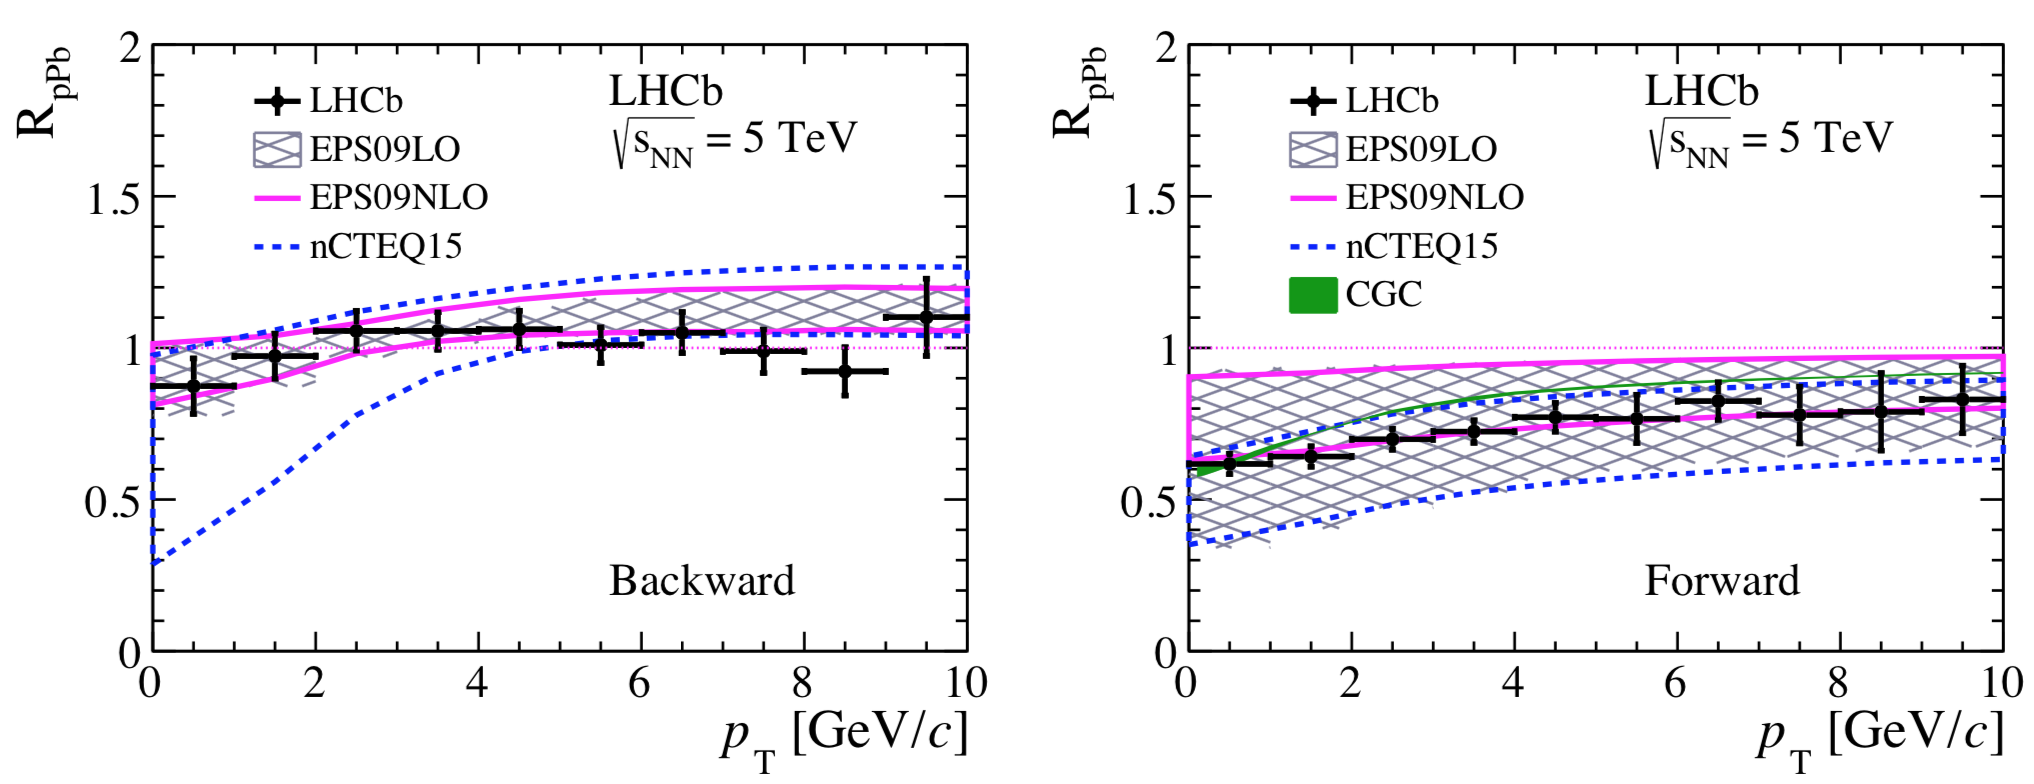
\includegraphics[width=.65\textwidth]{Plots/DRpAvsptLHCb2017}
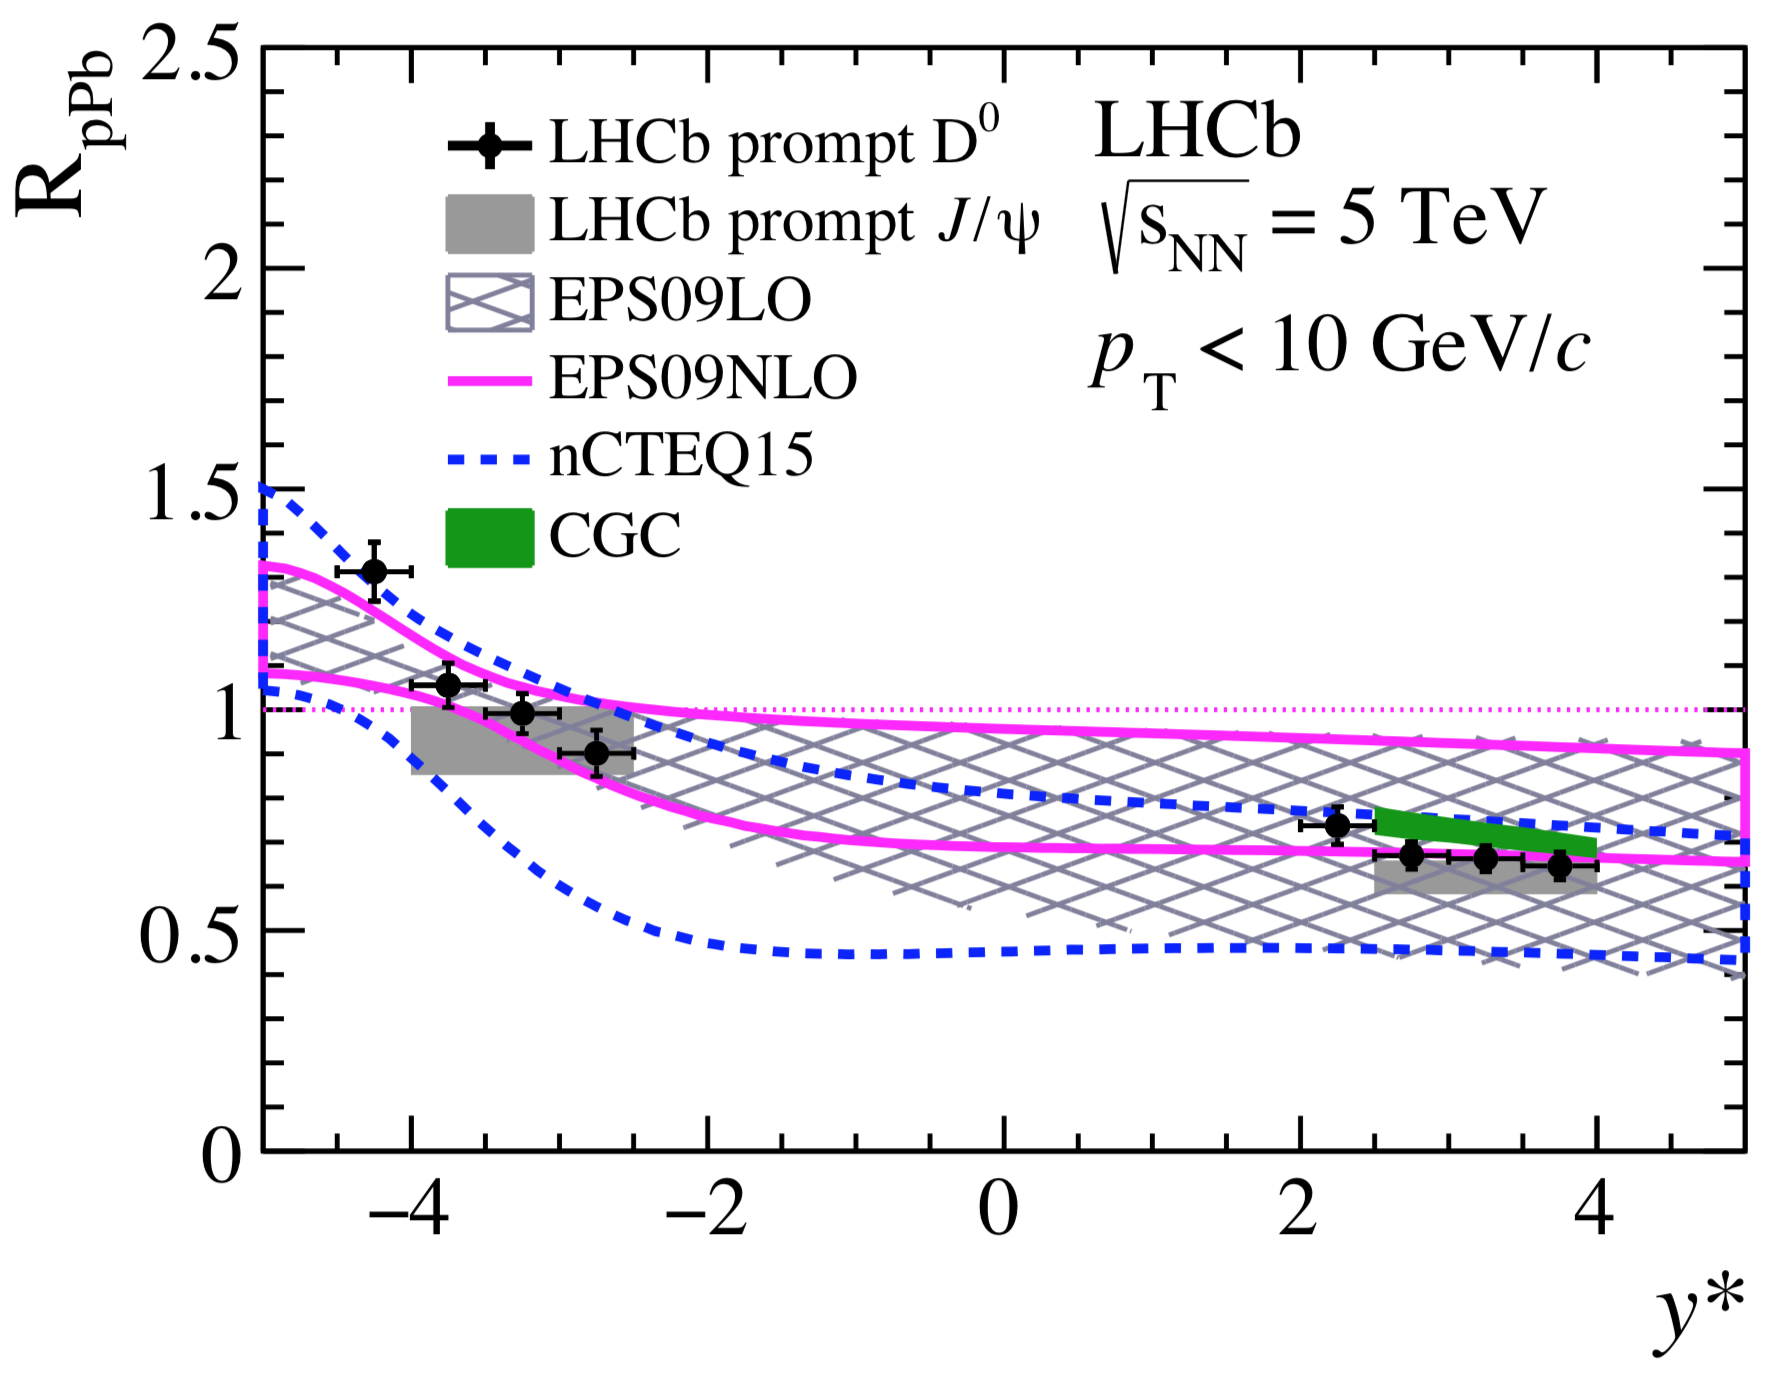
\includegraphics[width=.32\textwidth]{Plots/DRpALHCb2017}
%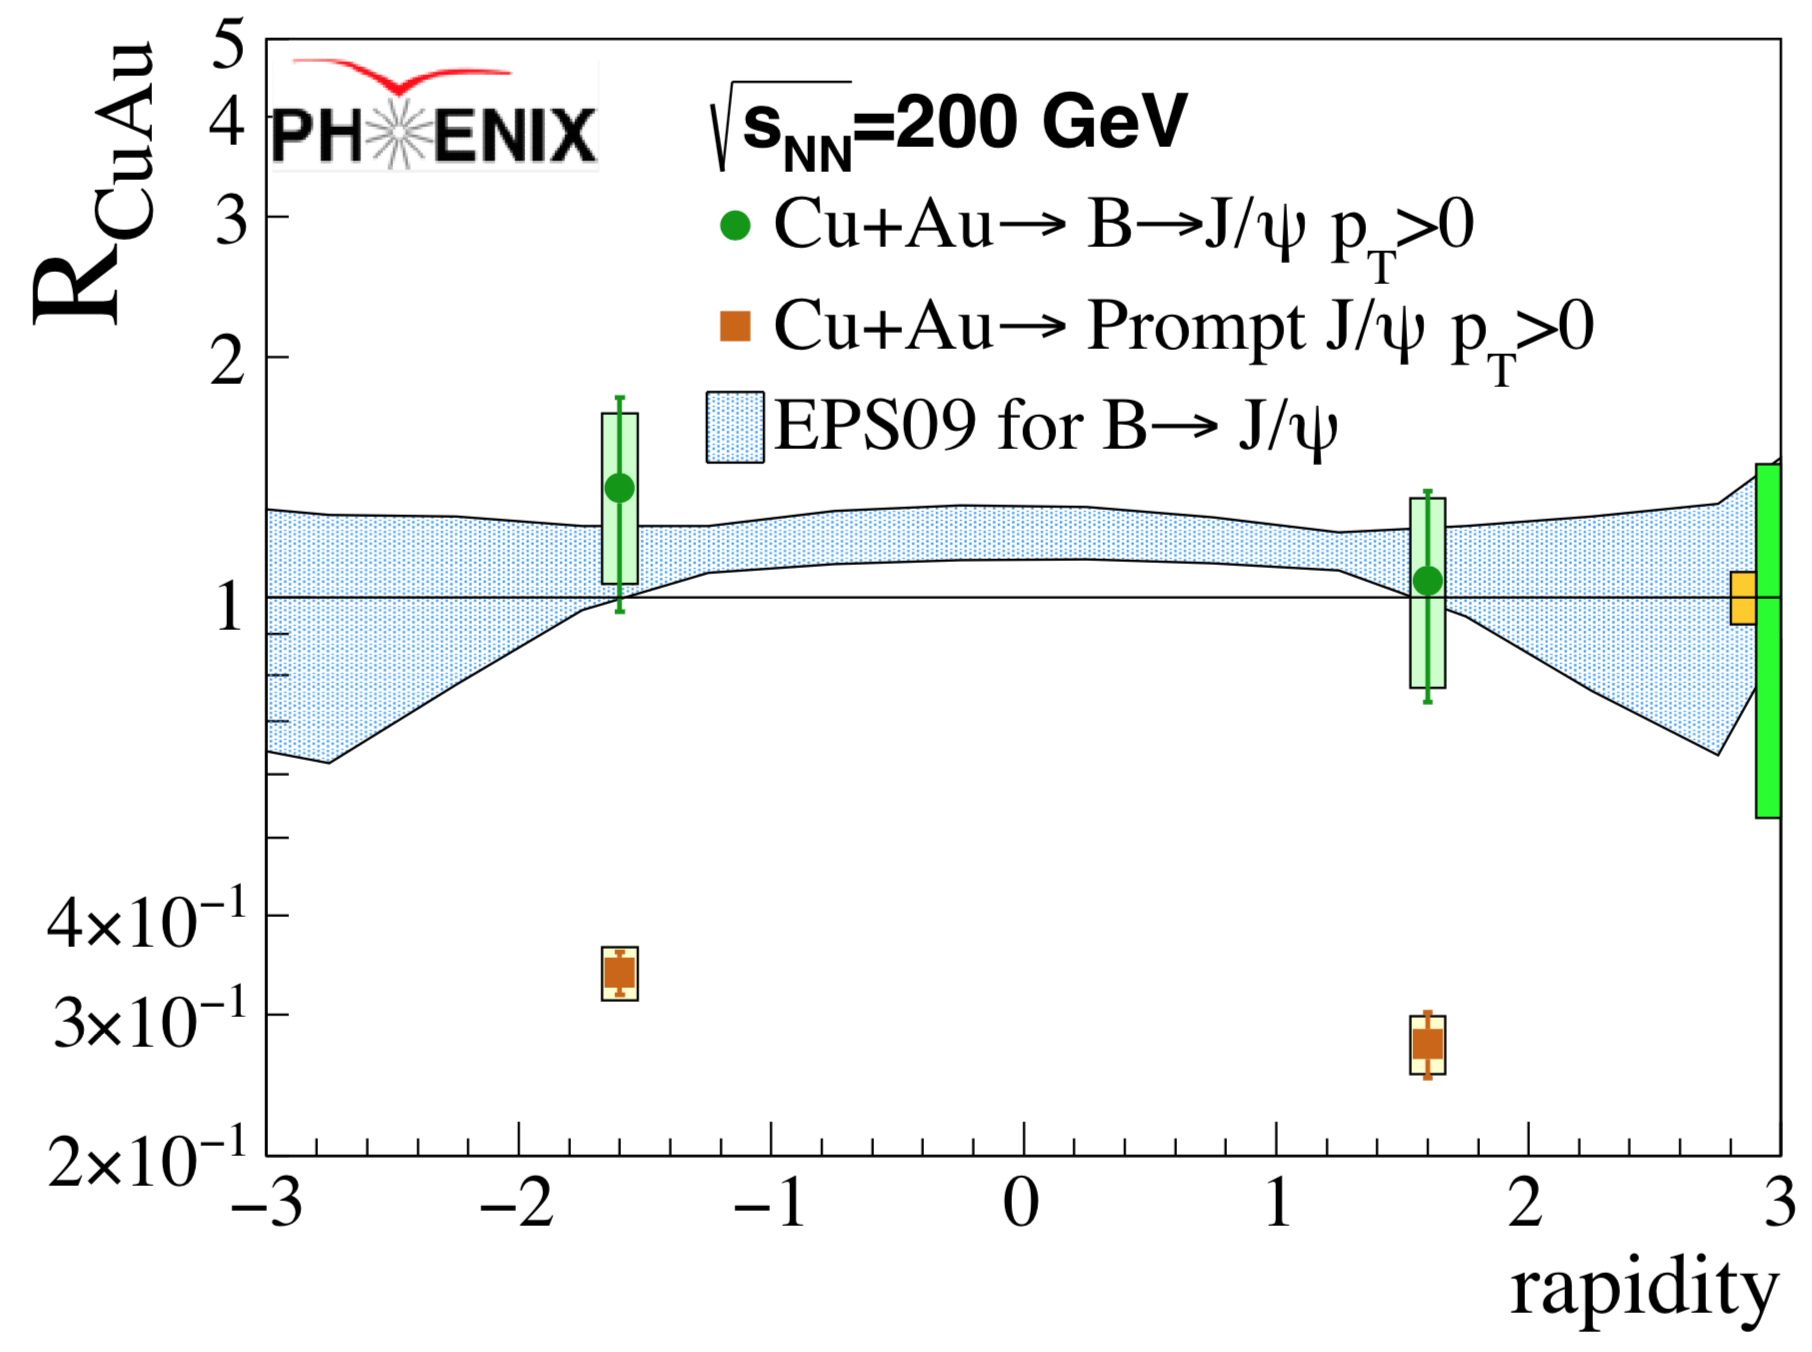
\includegraphics[width=.45\textwidth]{Plots/BRpAPHENIX}
\caption{Please write your figure caption here}
\label{RpA}     
\end{figure}


\begin{figure}[ht]
\centering
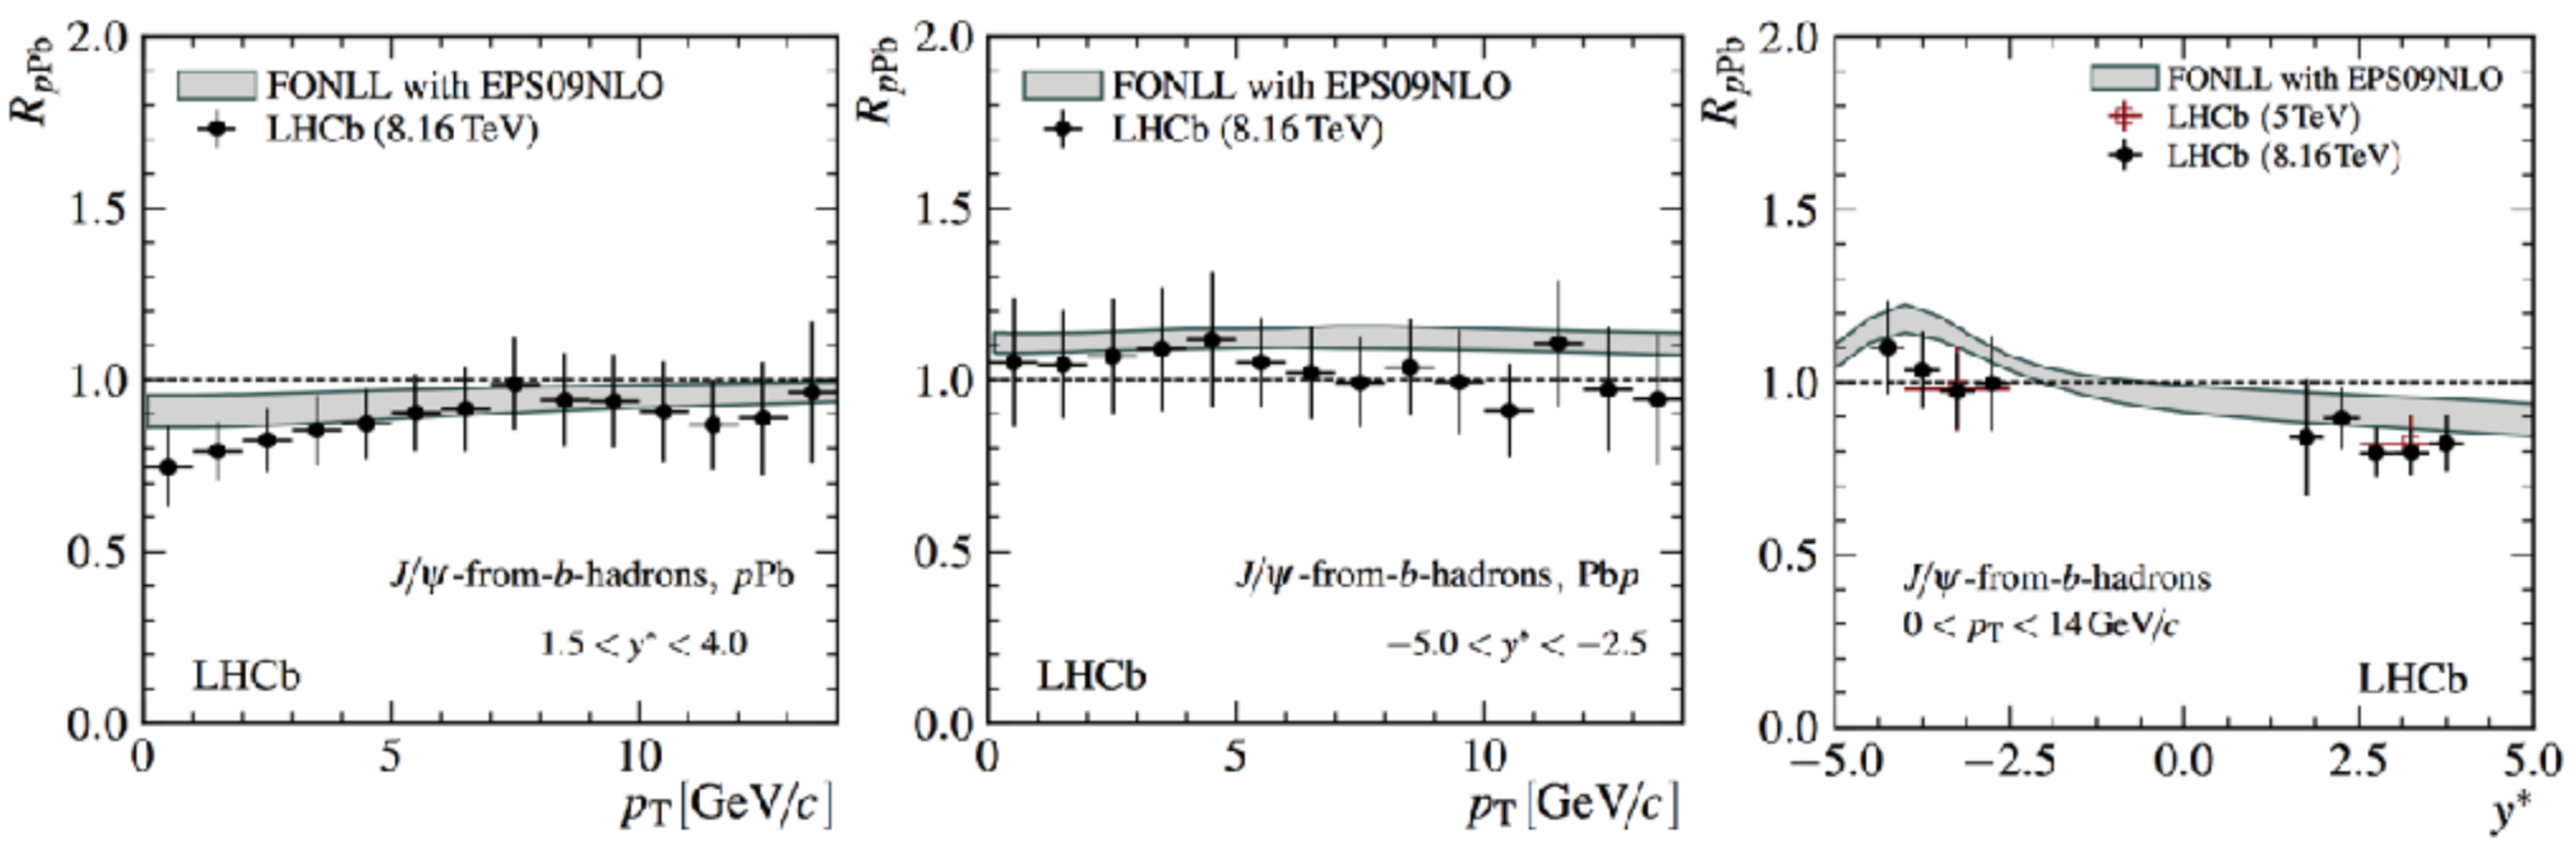
\includegraphics[width=.99\textwidth]{Plots/BRpAtLHC}
\caption{Please write your figure caption here}
\label{BRpA}     
\end{figure}


\begin{figure}[ht]
\centering
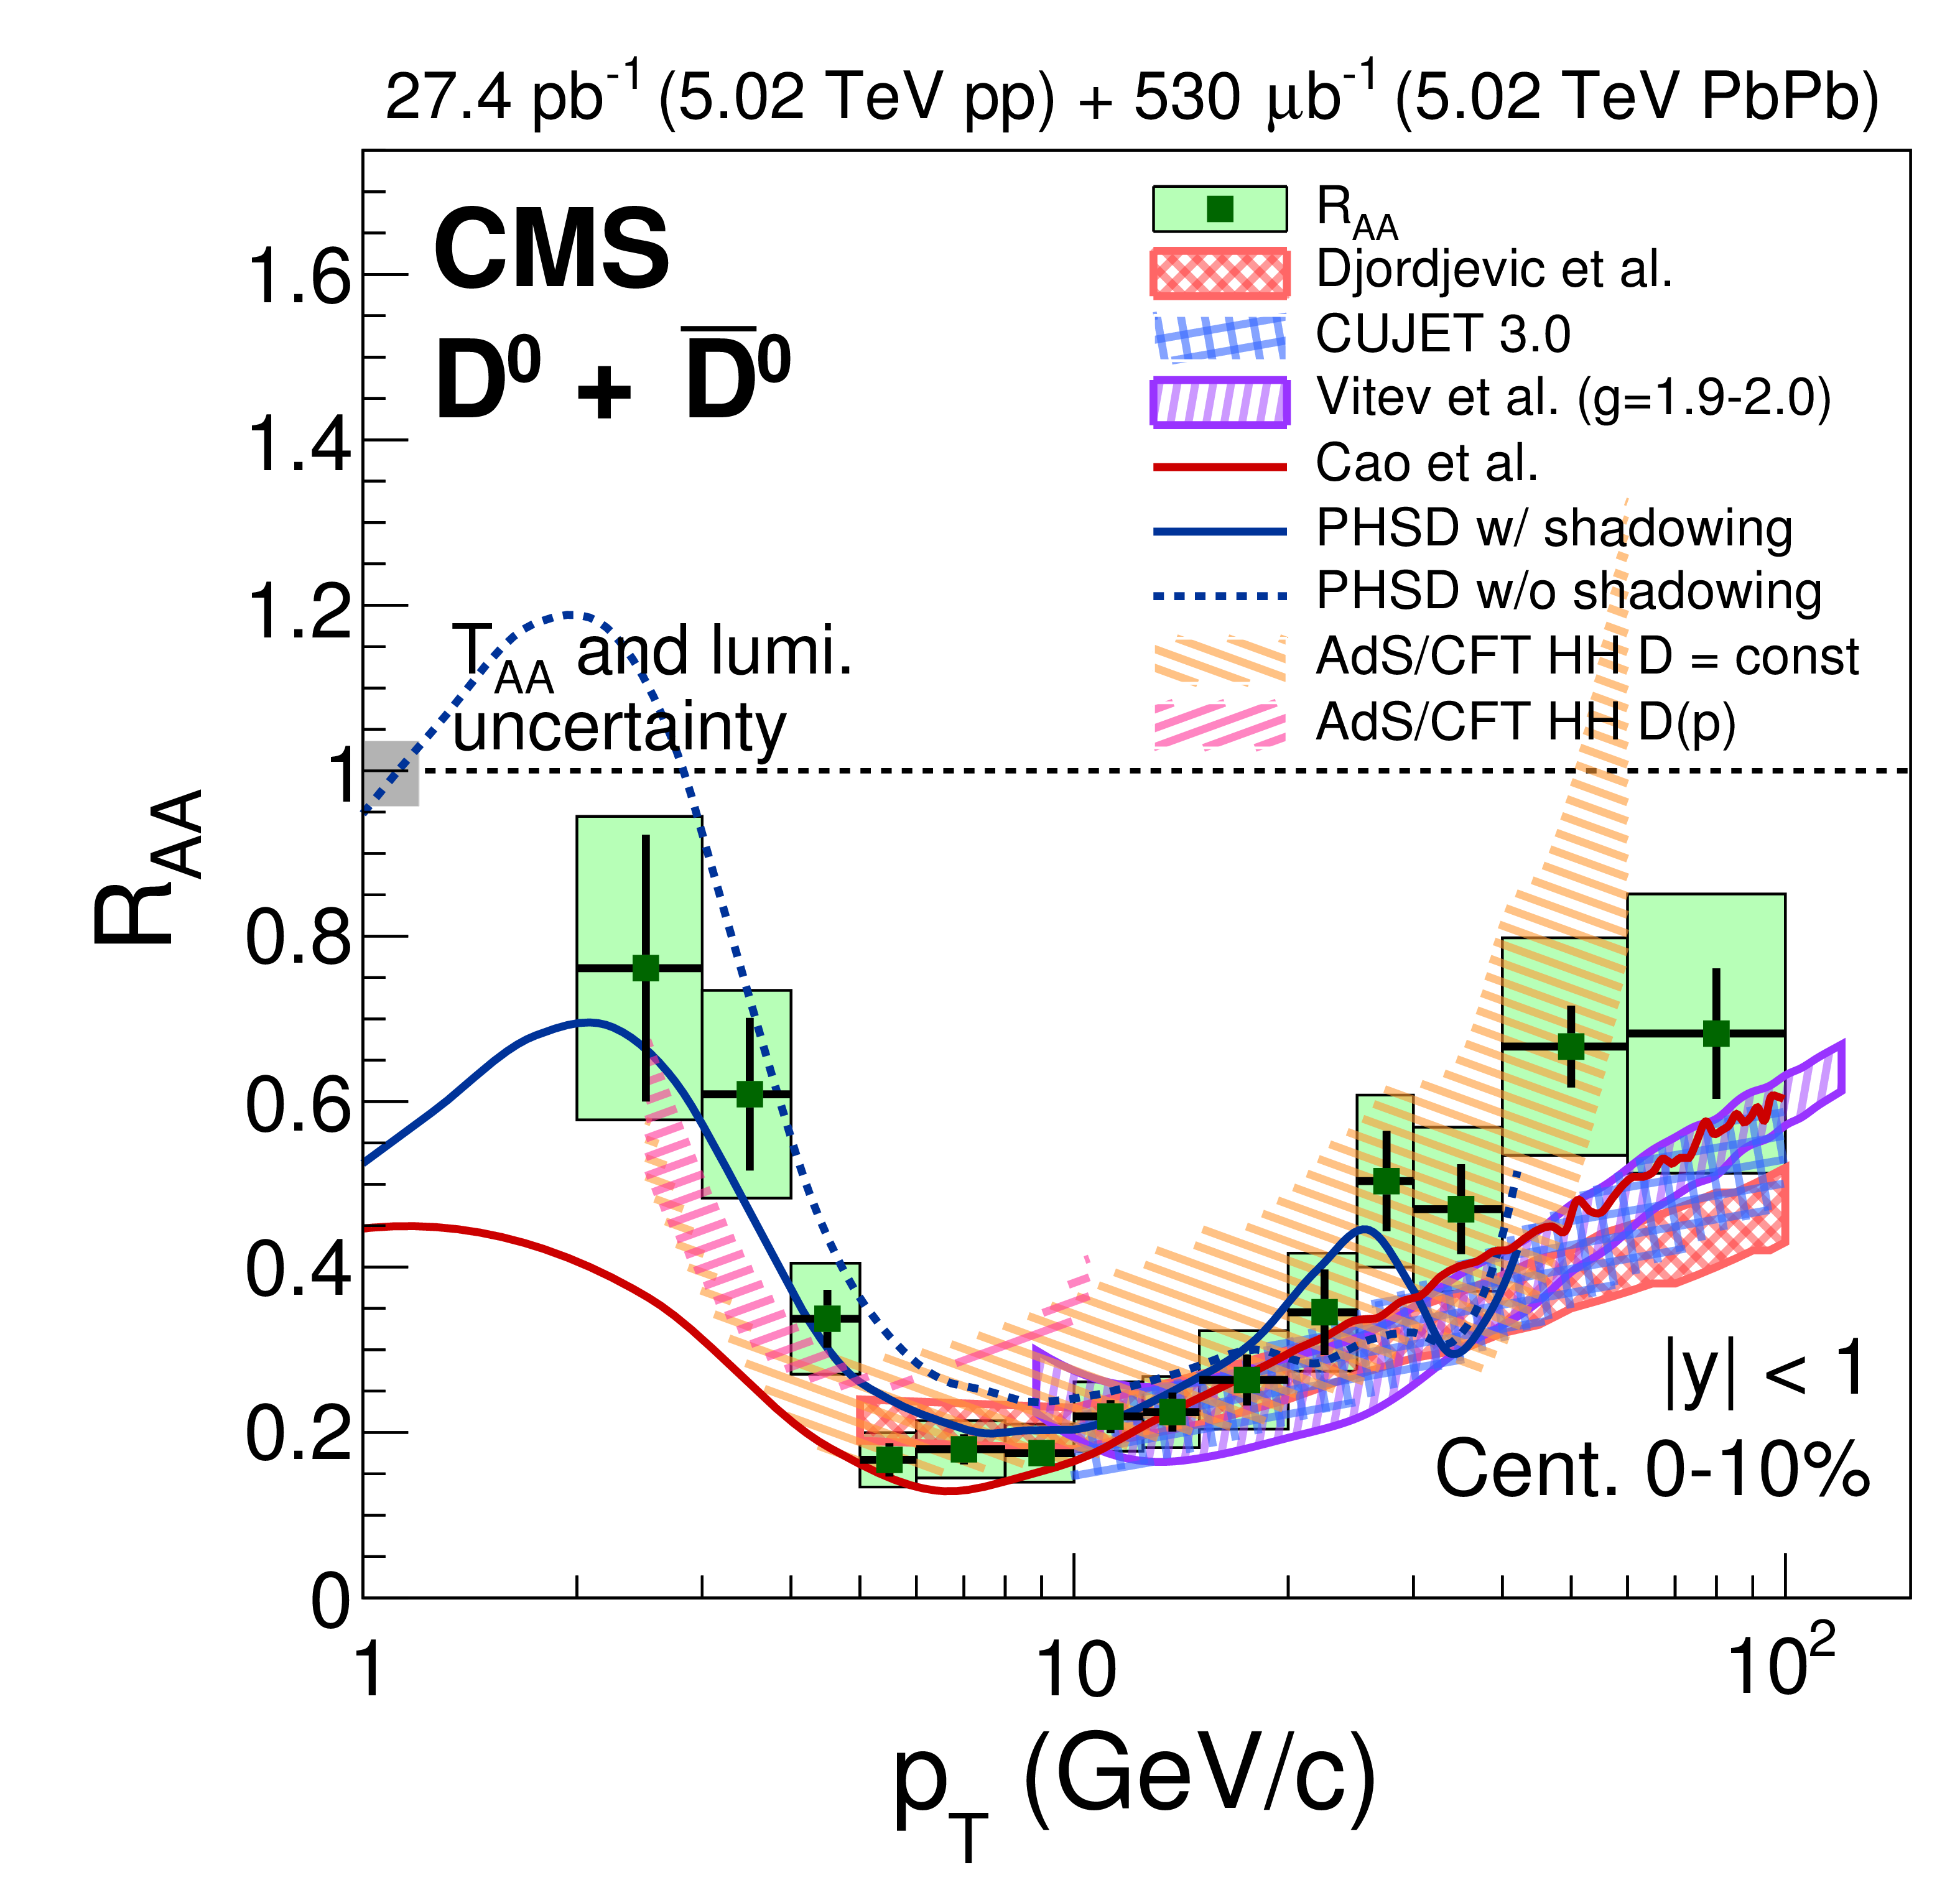
\includegraphics[width=.30\textwidth]{Plots/DRAACMS010}
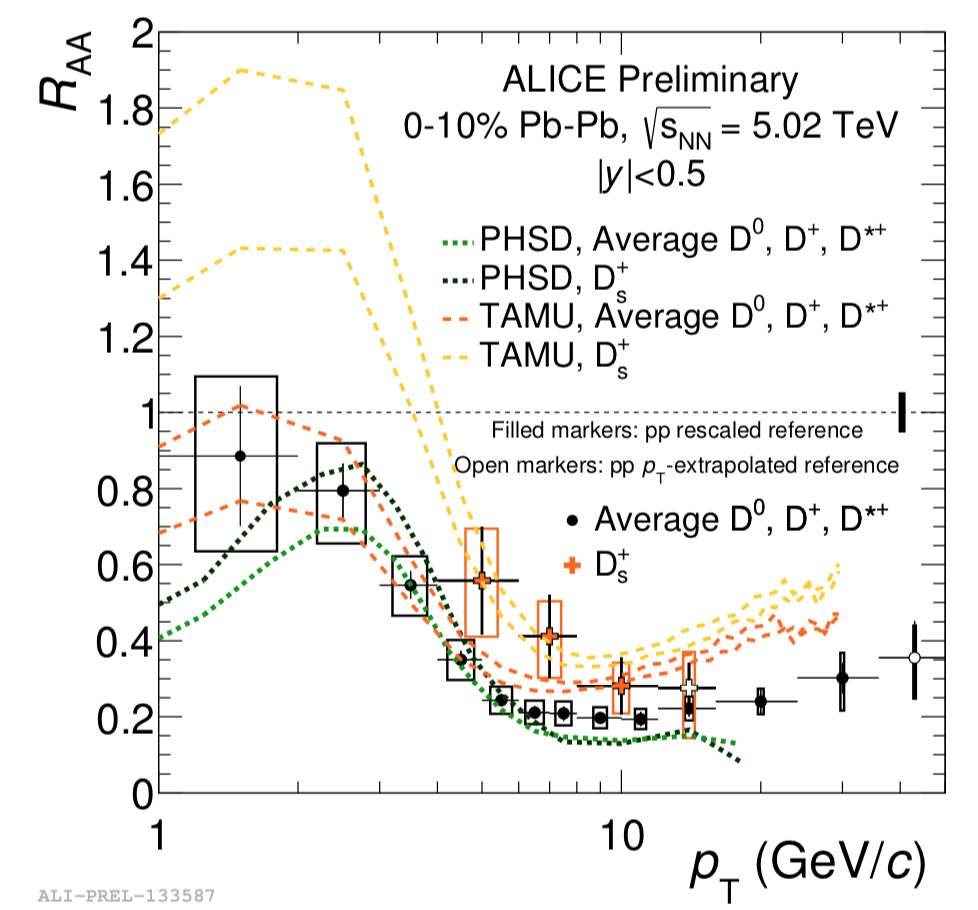
\includegraphics[width=.30\textwidth]{Plots/DmesonRAAALICE2017zoom}
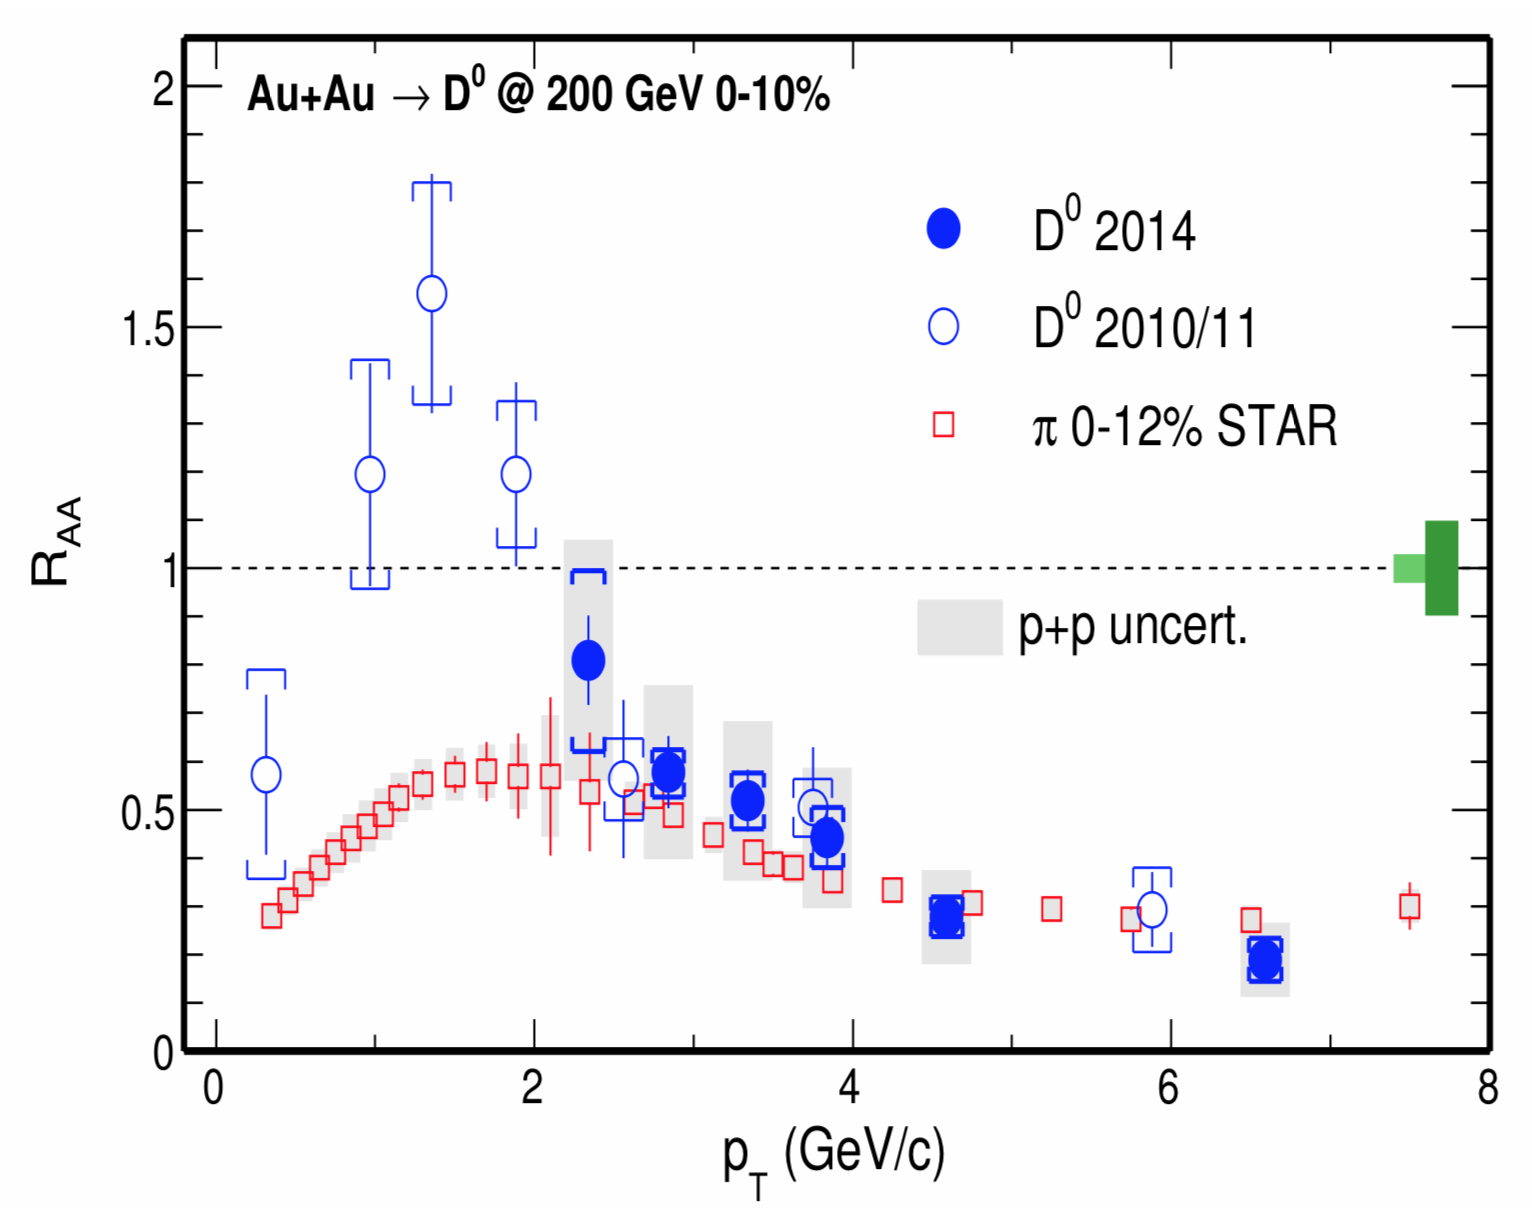
\includegraphics[width=.37\textwidth]{Plots/DRAASTARAuAu}

\caption{Please write your figure caption here}
\label{DRAA}     
\end{figure}

\begin{figure}[ht]
\centering
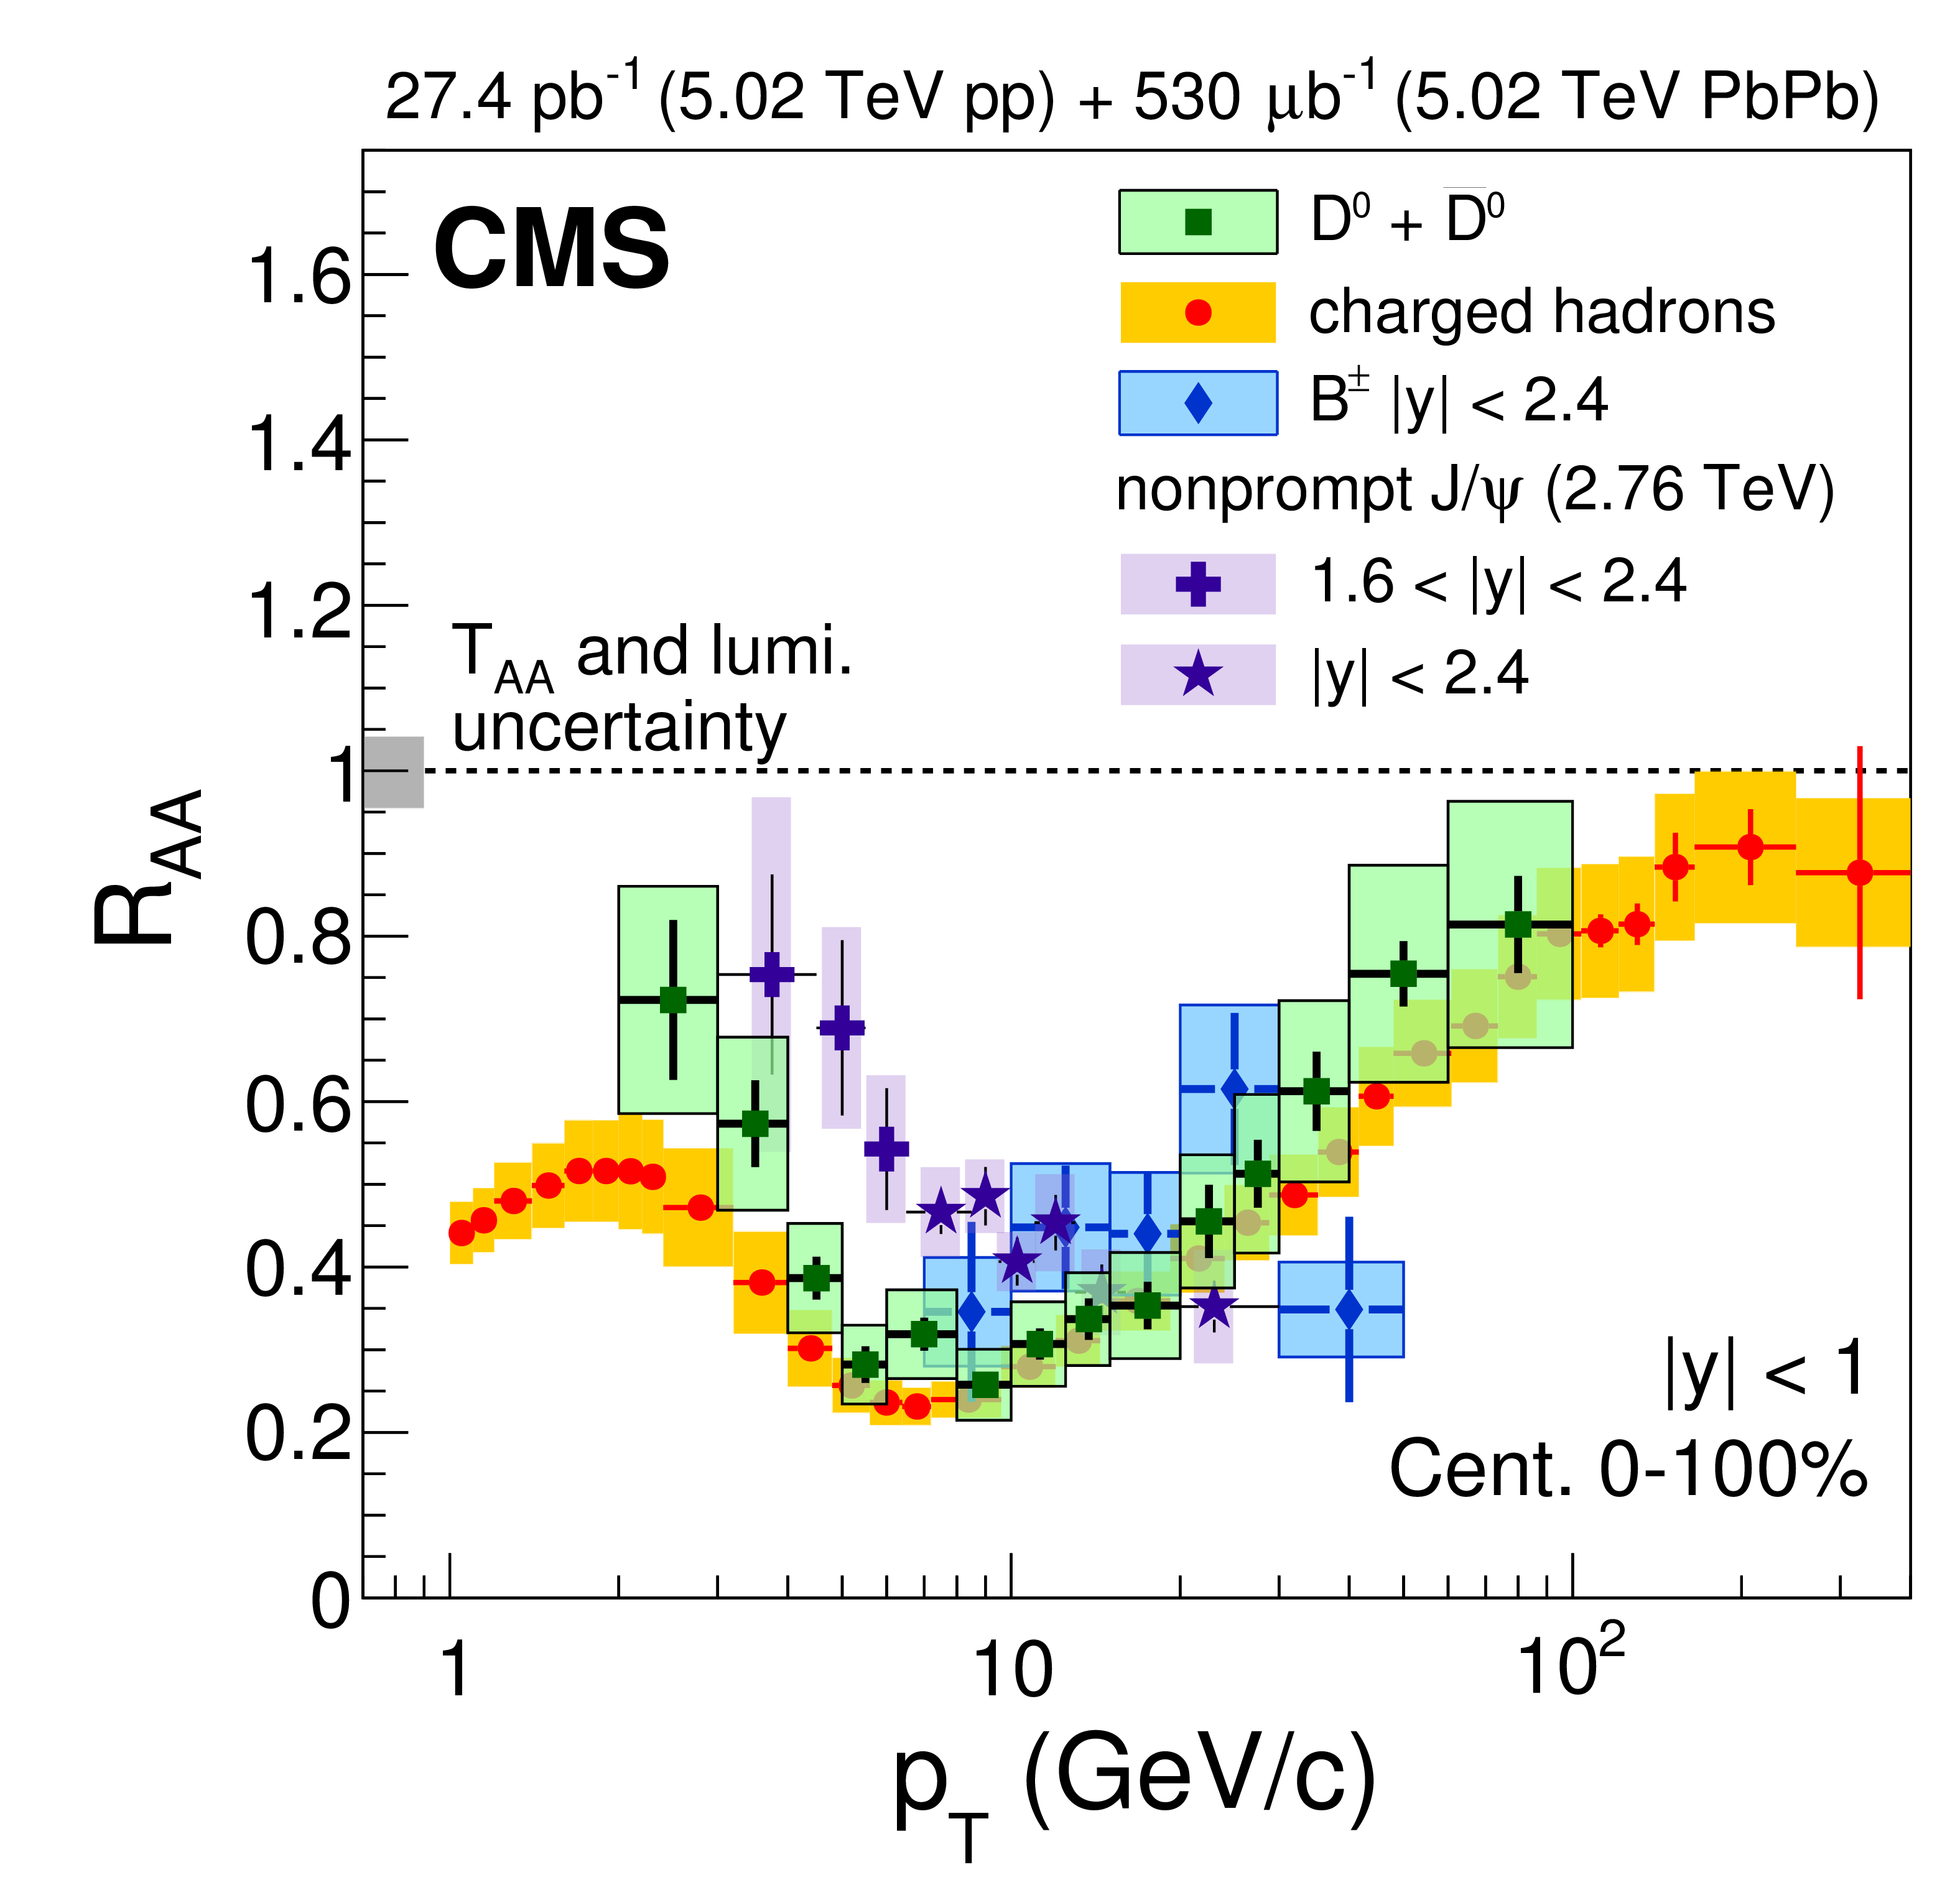
\includegraphics[width=.45\textwidth]{Plots/DBNonPromptRAACMS}
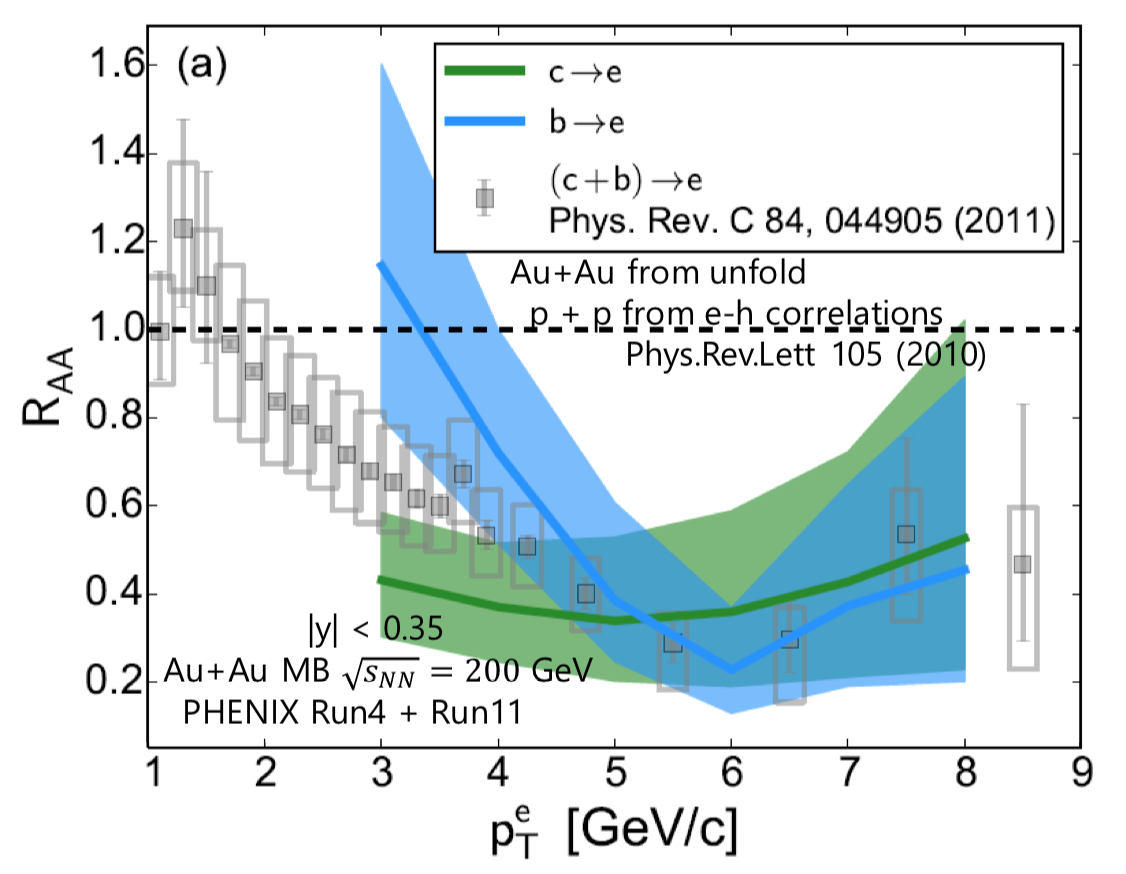
\includegraphics[width=.5\textwidth]{Plots/BPHENIXAuAu}
\caption{Please write your figure caption here}
\label{FlavourRAA}     
\end{figure}


\begin{figure}[ht]
\centering
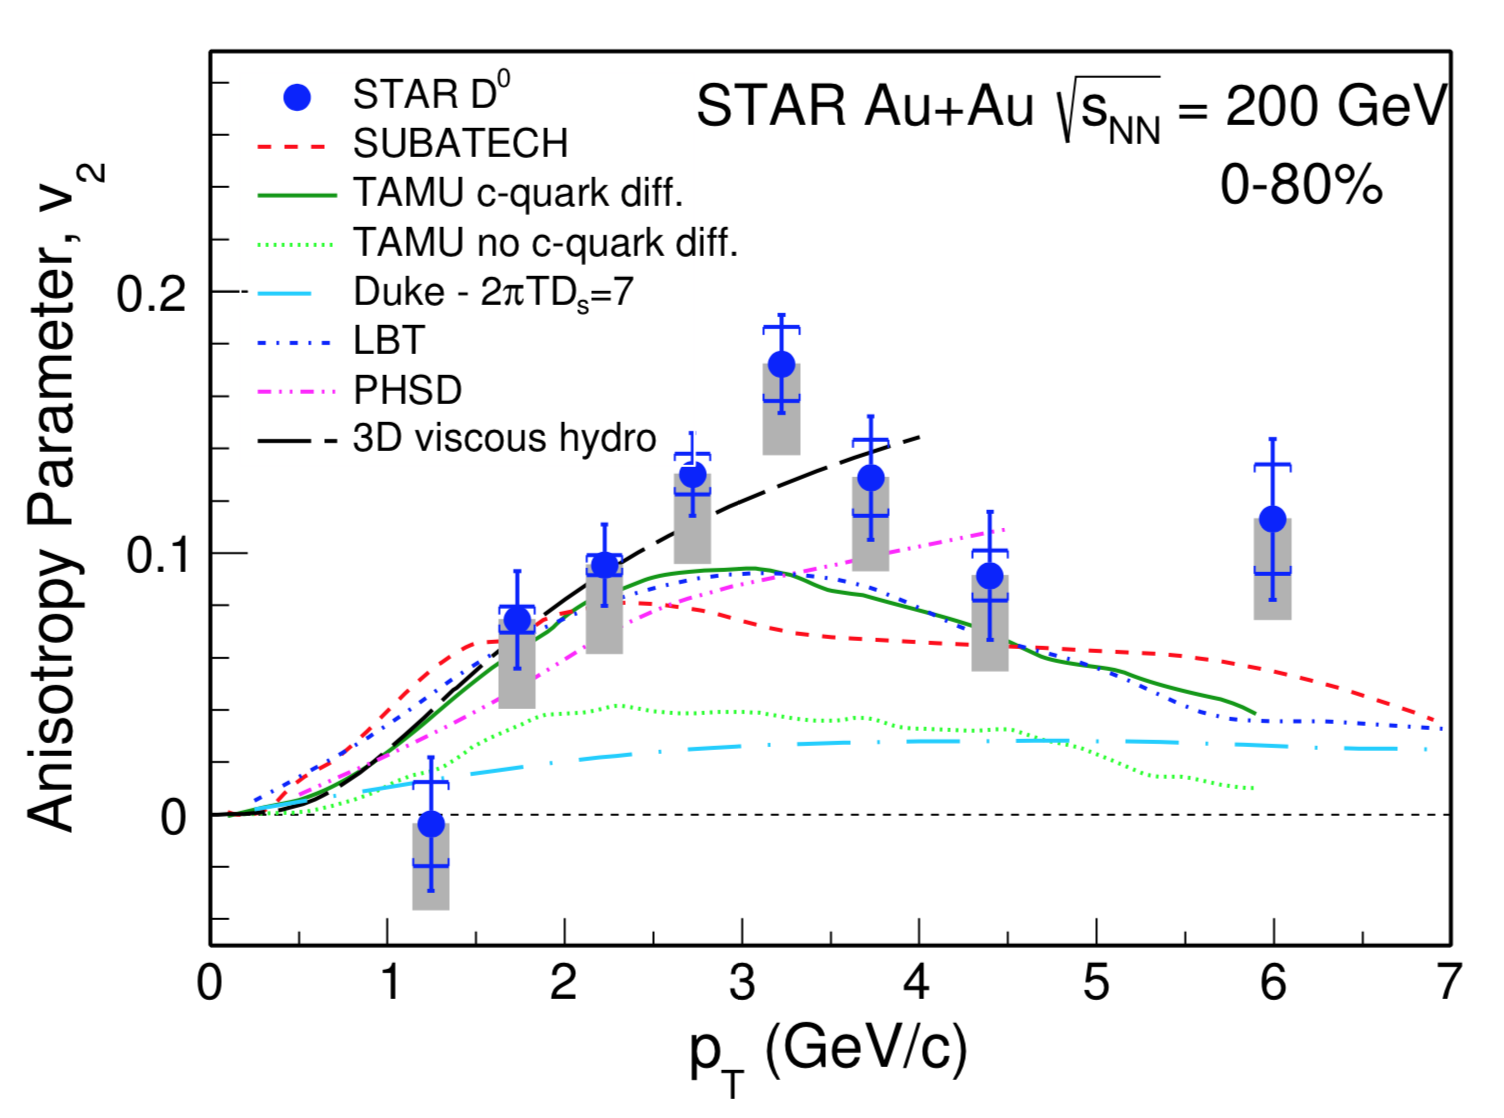
\includegraphics[width=.40\textwidth]{Plots/Dmesonv2STAR}
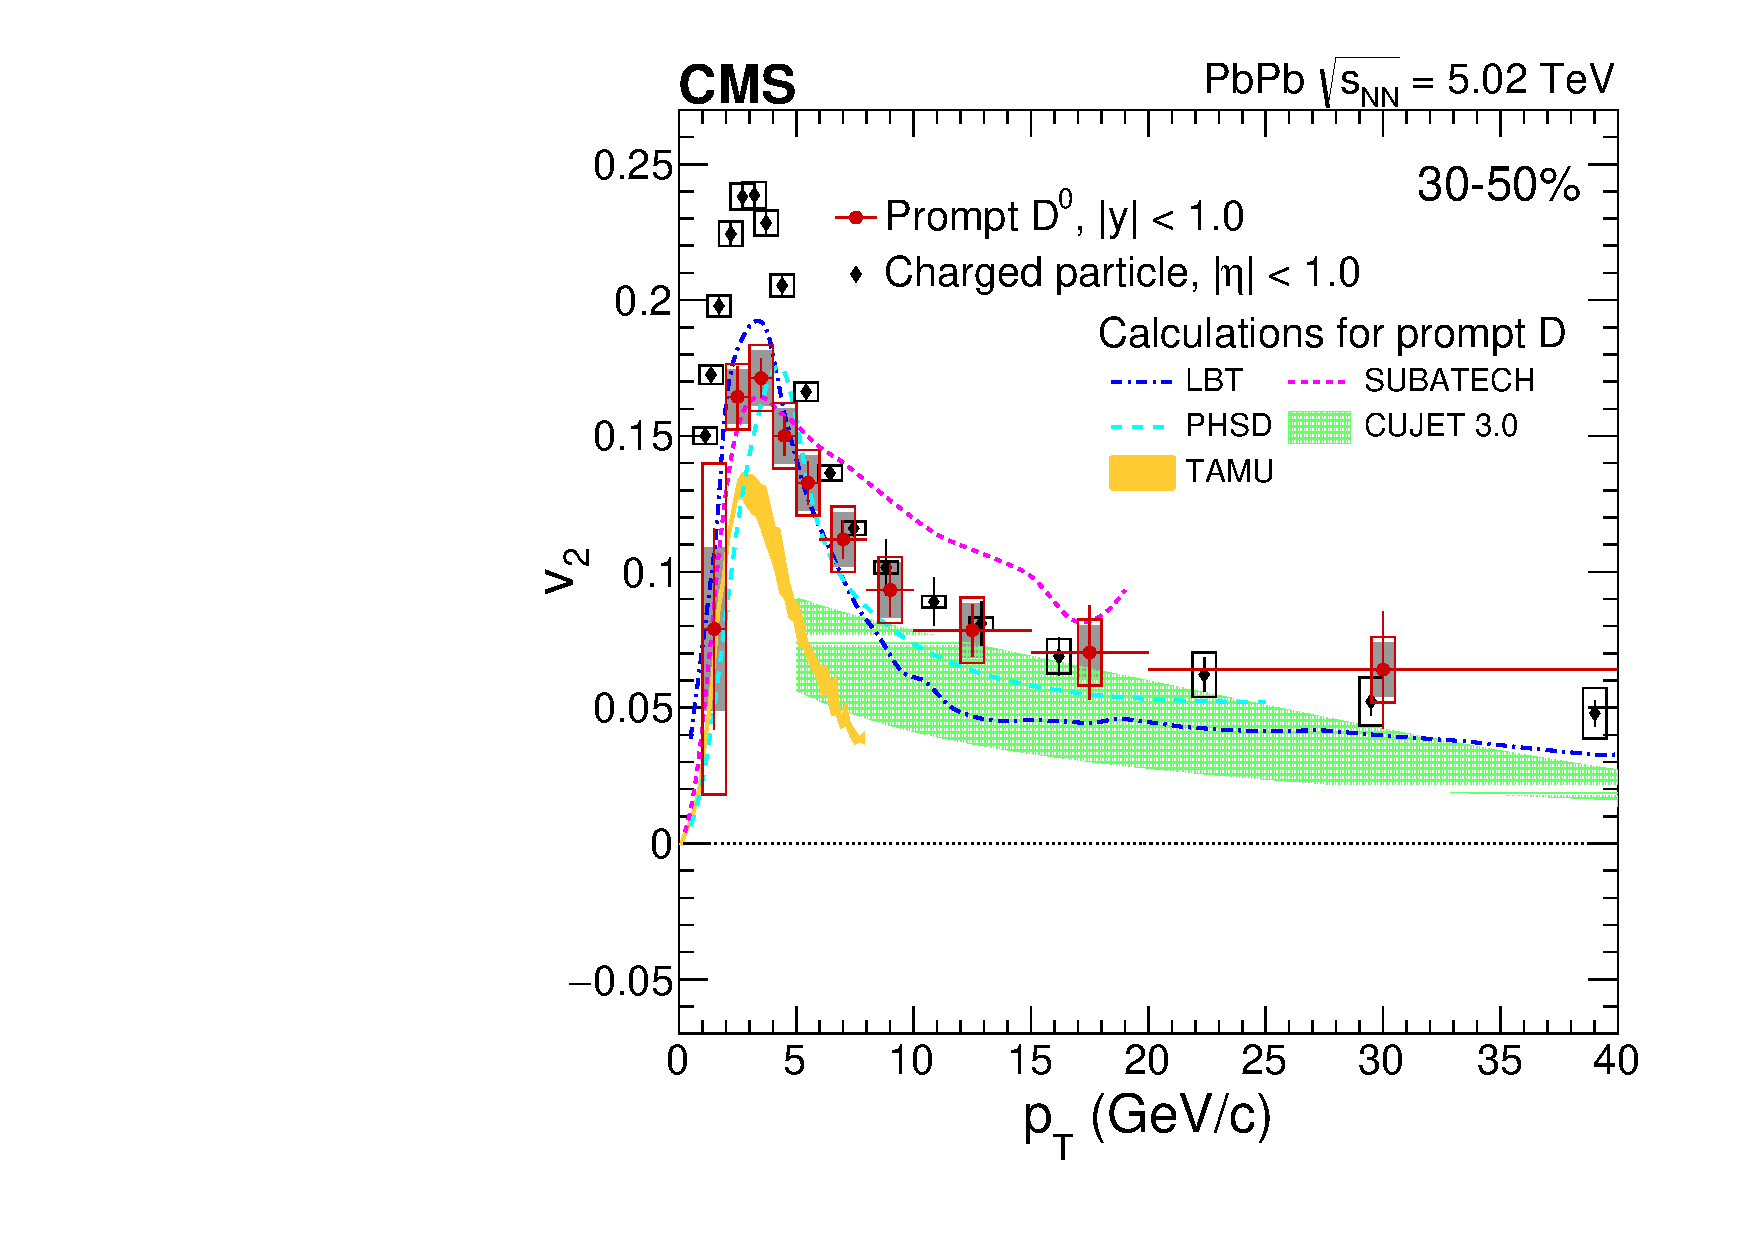
\includegraphics[width=.29\textwidth]{Plots/Dv2CMS3050.pdf}
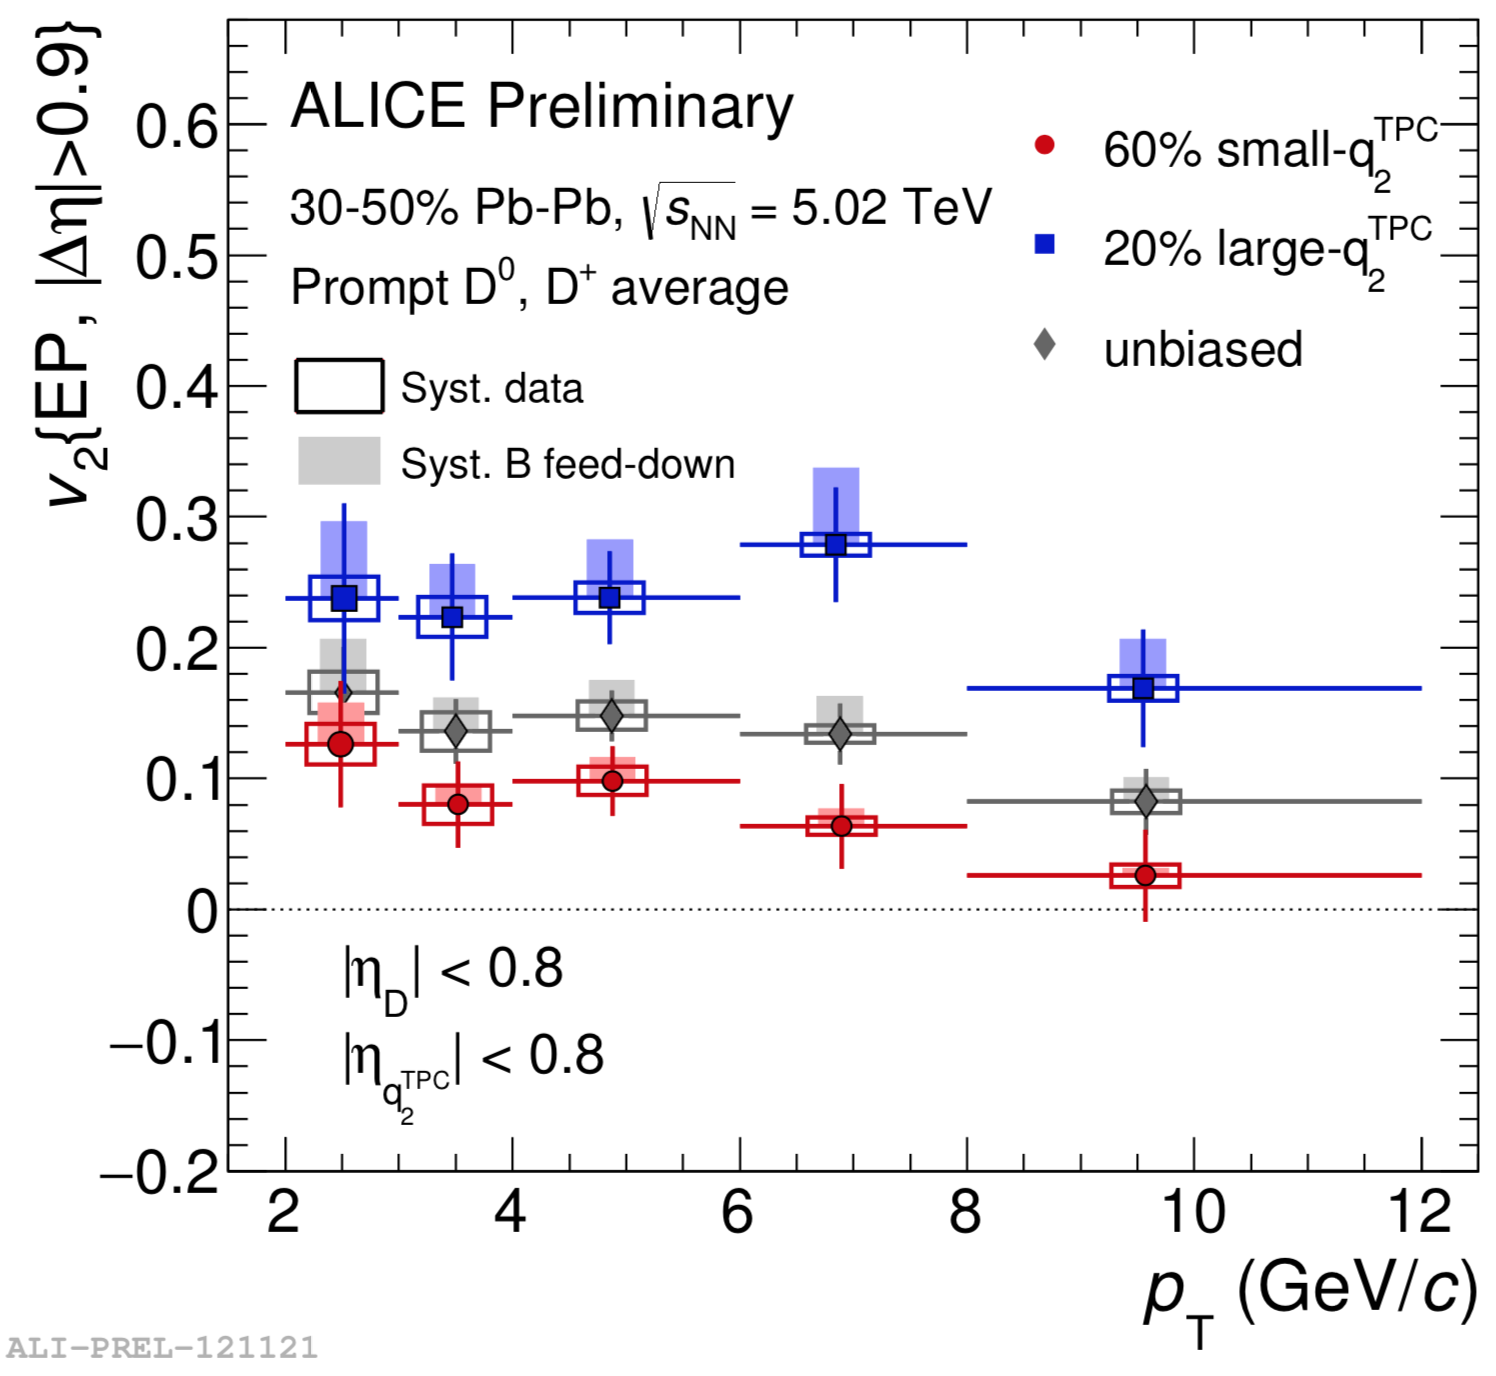
\includegraphics[width=.29\textwidth]{Plots/DmesonEventShapeALICEPbPb}
\caption{Please write your figure caption here}
\label{Dvn}     
\end{figure}

\begin{figure}[ht]
\centering
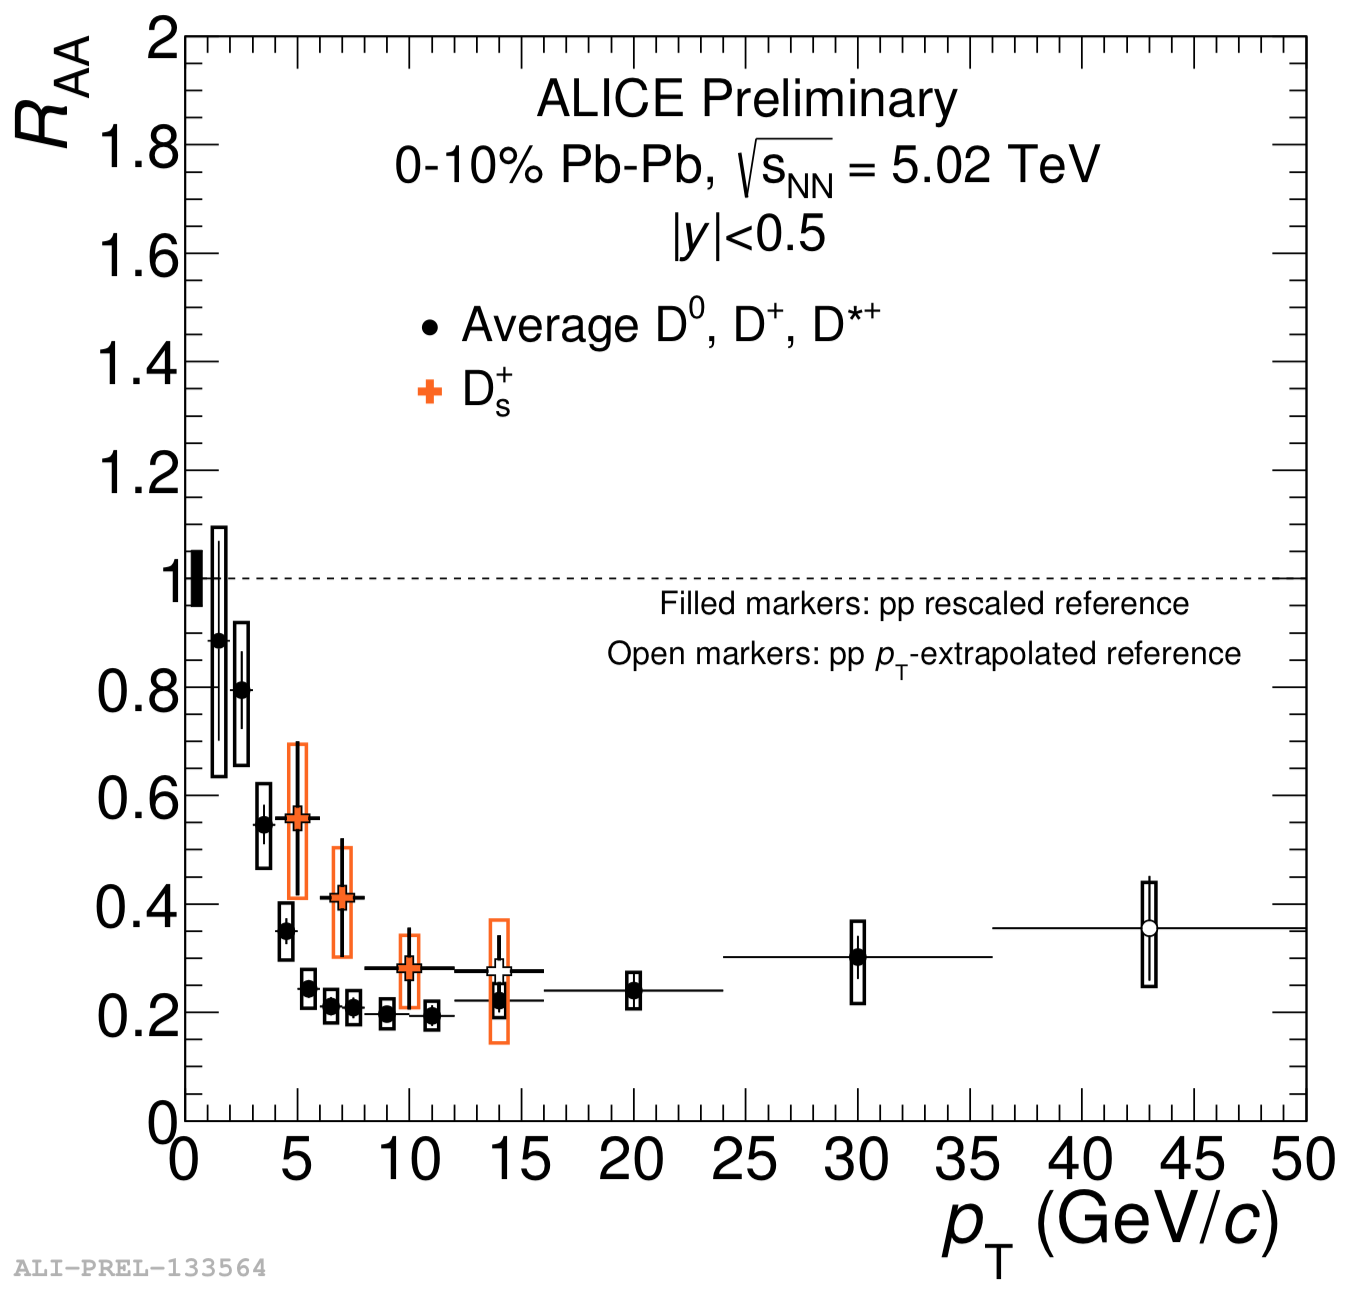
\includegraphics[width=.45\textwidth]{Plots/DsDRAA502TeV}
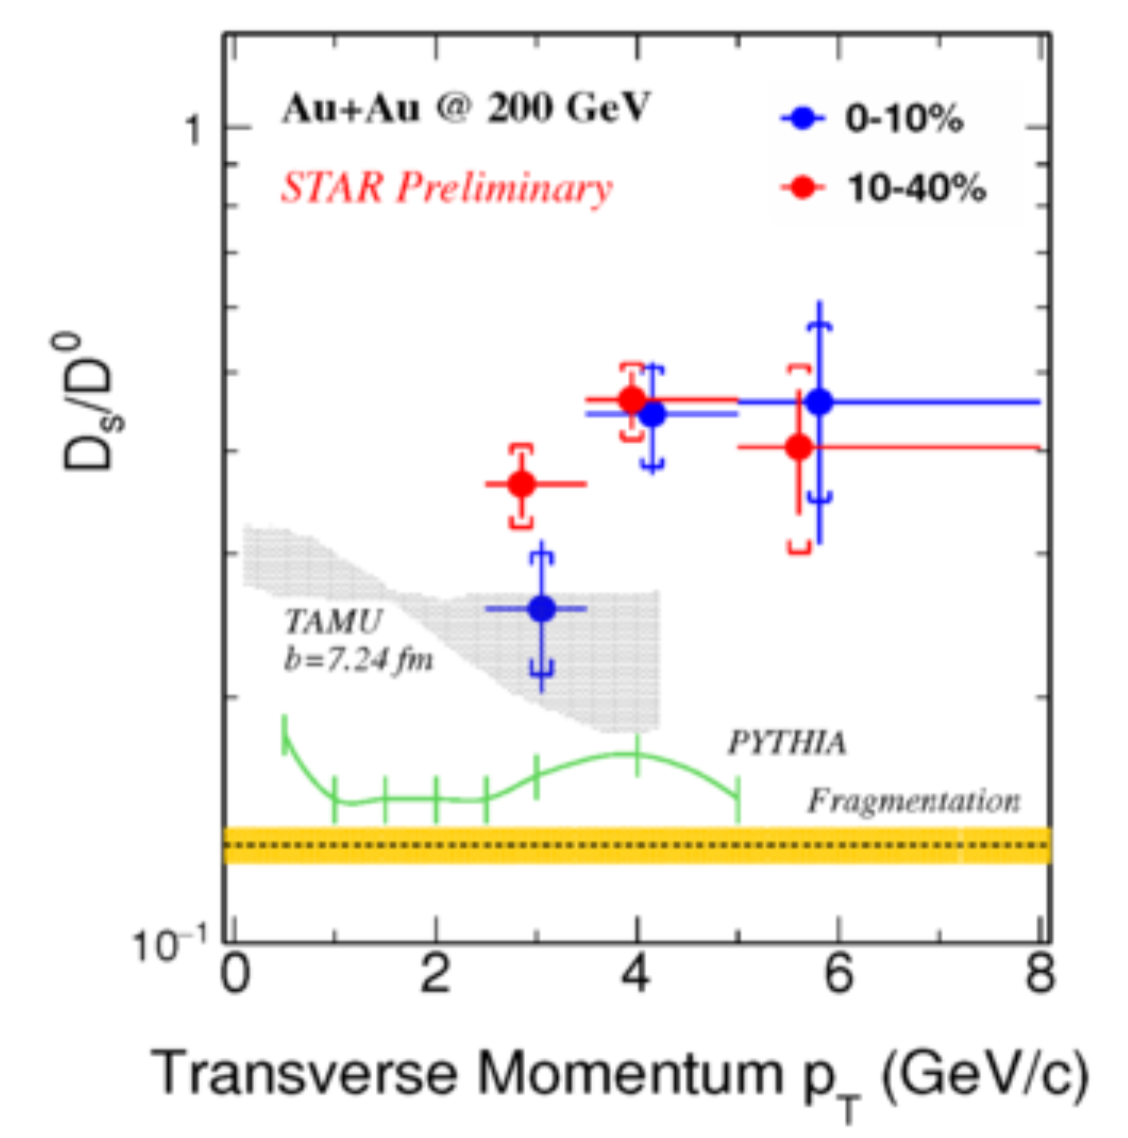
\includegraphics[width=.45\textwidth]{Plots/DsDSTARAuAu}
\caption{Please write your figure caption here}
\label{recombinationMesons}     
\end{figure}

\begin{figure}[ht]
\centering
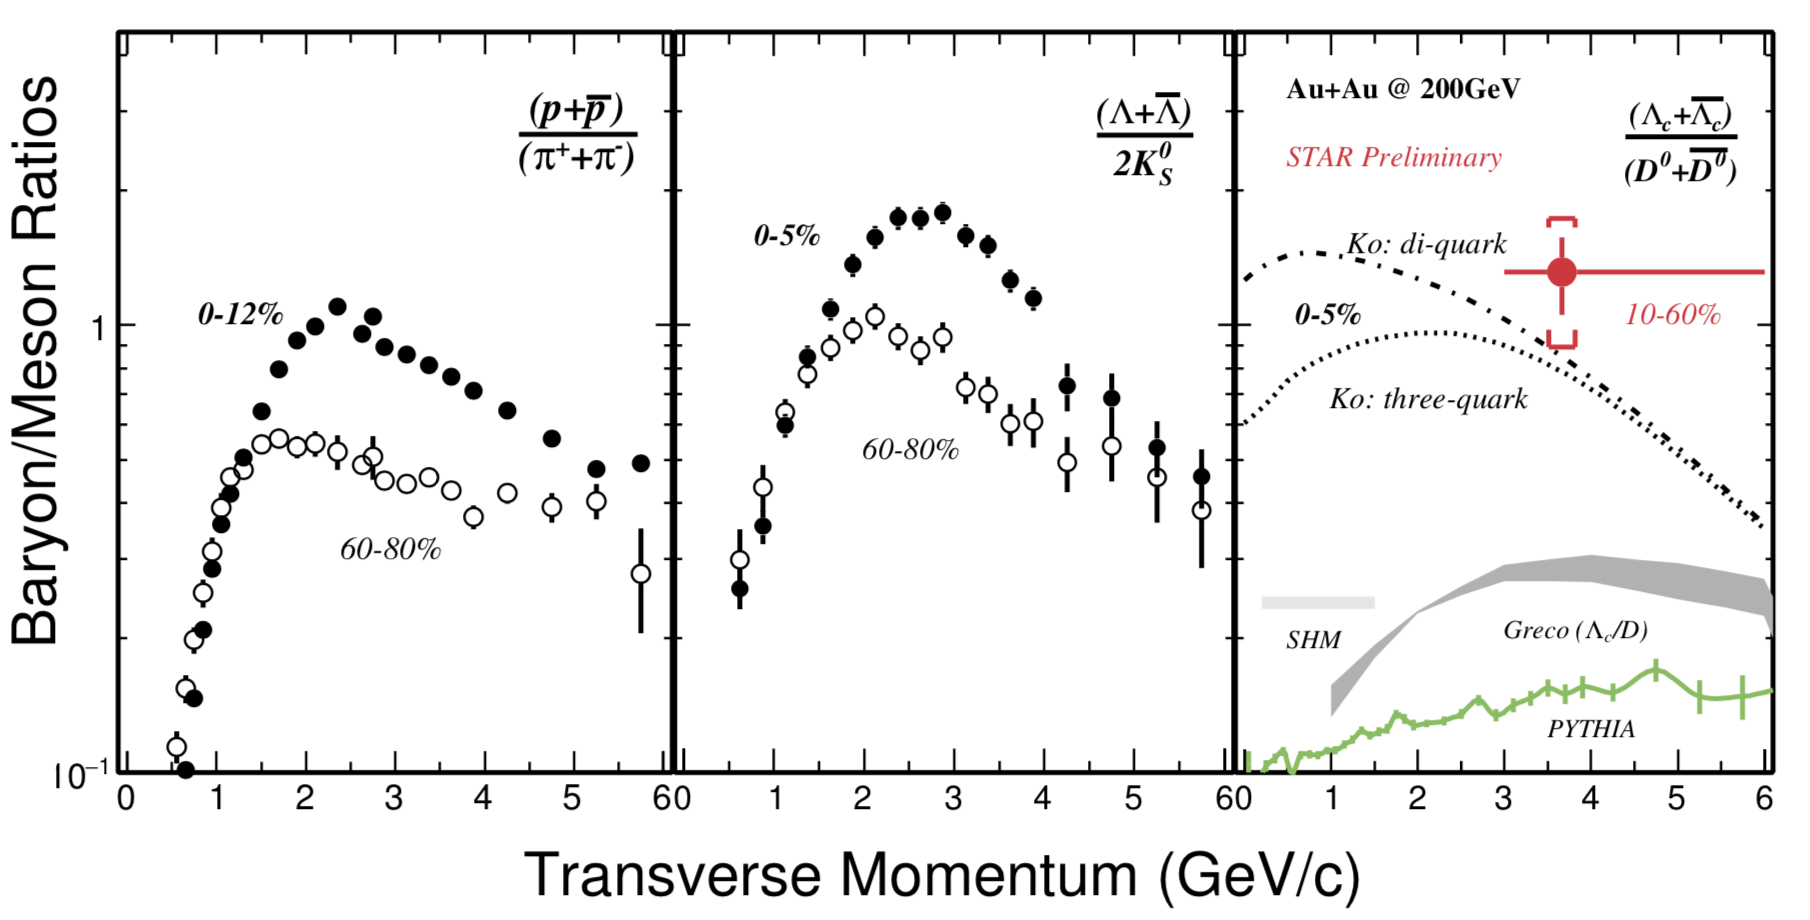
\includegraphics[width=.90\textwidth]{Plots/LambdacSTARAuAu}
\caption{Please write your figure caption here}
\label{recombinationBaryons}     
\end{figure}


%%%%%%%%%%%%%%%%%%%%%%%%%
\begin{thebibliography}{}
\bibitem{saporegravis} A. Andronic et al., Eur. Phys. J. C 76 (2016) 107, doi:10.1140/epjc/s10052-015-3819-5, arXiv:1506.03981. 
\end{thebibliography}
\end{document}

\end{figure}


% end of file template.tex

%<div id='footer'><table width='100%'><tr><td class='right'><a href='http://fusioninventory.org/'><span class='copyright'>FusionInventory 9.1+1.0 | copyleft <img src='/glpi/plugins/fusioninventory/pics/copyleft.png'/>  2010-2016 by FusionInventory Team</span></a></td></tr></table></div>